 \documentclass{template/openetcs_article}
%\documentclass{article}
%\usepackage[ascii]{inputenc}
%\usepackage[T1]{fontenc}
\usepackage[english]{babel}
\usepackage{amsmath}
\usepackage{amssymb,amsfonts,textcomp}
\usepackage{array}
\usepackage{supertabular}
\usepackage{hhline}
\usepackage{graphicx}
\usepackage{lscape}
\usepackage{float}
\usepackage{url}
\usepackage{hyperref}
\usepackage{breakurl}
\usepackage{lipsum}
\makeatletter
\newcommand\arraybslash{\let\\\@arraycr}
\makeatother
\setlength\tabcolsep{1mm}
\renewcommand\arraystretch{1.3}
\newcounter{Ilustracin}
\renewcommand\theIlustracin{\arabic{Ilustracin}}
\title{openETCS}

%\setcounter{tocdepth}{3}

\usepackage{hhline}
\usepackage{booktabs}
\usepackage{multirow}
\usepackage{color, colortbl}
\definecolor{myblue}{rgb}{0.6,.6,1}
\definecolor{mydarkblue}{rgb}{0,0,0.5}
\definecolor{mylightblue}{rgb}{0.8,0.8,1}
\usepackage{hyperref}
\hypersetup{colorlinks=true, linkcolor=mydarkblue, urlcolor=mydarkblue}




%%%%% comments %%%%%
% To allow MS Word style comments at the document margin we use the todonotes package. A comment is made as follows:

%\mycomment[IN]{text}

% The text in brackets should be your initials and the text in curly braces is your actual comment. Comments are numbered automatically. 
\usepackage[textwidth=2.7cm,textsize=scriptsize,linecolor=green!40,backgroundcolor=green!40]{todonotes}

\newcounter{mycommentcounter}
\newcommand{\mycomment}[2][]
{
\refstepcounter{mycommentcounter}%
\todo[color={red!100!green!33}]{
\textbf{[\uppercase{#1} \themycommentcounter]:} #2}
}


% Use the option "nocc" if the document is not licensed under Creative Commons
%\documentclass[nocc]{template/openetcs_article}
\usepackage{lipsum,url}
\graphicspath{{./template/}{.}{./images/}}
\begin{document}
\frontmatter
\project{openETCS}

%Please do not change anything above this line
%============================
% The document metadata is defined below

%assign a report number here
\reportnum{OETCS/WP1/D1.3.1}

%define your workpackage here
\wp{Work-Package 1: ``Management''}

%set a title here
\title{Project Quality Assurance Plan}

%set a subtitle here
%\subtitle{A template for short document. Adapted from report template.}

%set the date of the report here
\date{\today}

%define a list of authors and their affiliation here

\author{Izaskun de la Torre}

\affiliation{SQS \\Avenida Zugazarte 8 \\
  48930 Getxo, Spain}


% define the coverart
\coverart[width=350pt]{openETCS_EUPL}

%define the type of report
\reporttype{Description of work}




%=============================
%Do not change the next three lines
\maketitle
\tableofcontents
\listoffiguresandtables
\newpage
%=============================

% The actual document starts below this line
%=============================


%Start here



%\begin{document}


\section*{Document History}

\begin{center}
\begin{longtable}{m{1.1cm}m{1.8cm}m{2cm}m{5cm}m{4cm}}
\caption{Documentation History}\\

\hline \rowcolor{myblue} \multicolumn{1}{l}{Version} & \multicolumn{1}{l}{Date} & \multicolumn{1}{l}{Chapters modified} & \multicolumn{1}{l}{Reason} & \multicolumn{1}{l}{Name} \\ \hline 
\endfirsthead

\multicolumn{5}{c}%
{{\bfseries \tablename\ \thetable{} -- continued from previous page}} \\
\hline \rowcolor{myblue} \multicolumn{1}{l}{Version} & \multicolumn{1}{l}{Date} & \multicolumn{1}{l}{Chapters modified} & \multicolumn{1}{l}{Reason} & \multicolumn{1}{l}{Name} \\ \hline 
\endhead

\hline \hline
\endlastfoot

0.0.0 &
15.11.2012 &
All &
First Steps on frame evaluation &
Rico Kaseroni (DB)

Peyman Farhangi (DB)\\\hline
0.1.0 &
27.11.2012 &
All &
First Steps on Content &
Rico Kaseroni (DB)

Jan Welte (TUBS)

Peyman Farhangi (DB)

Matthias Kuhn (DB)\\\hline
0.1.1 &
29.11.2012 &
All &
Optimaziation of document structure, Revision of Chapters according to EN 50128, Merging with project specific tasks &
Stephan Jagusch (AEbt)

Rico Kaseroni (DB)

Cyril Cornu (All4tec)\\\hline

0.2.0 &
30.11.2012 &
Baseline Requirements for certification  &
Extention of Chapter according to EN 50128 &
Jan Welte (TUBS)

Rico Kaseroni (DB)\\\hline
0.3.0 &
19.12.2012 &
All &
Extention of Chapter 

0, 1, 2, 3 &
All4Tech, DB, SQS\\\hline
0.4.0 &
11.01.2013 &
All &
Extention to existing and further Chapters  &
All4Tech, DB, SQS\\\hline
0.6.0 &
28.01.2013 &
All &
IP Clean &
Rico Kaseroni (DB)

Cyril Cornu (All4tec)\\\hline
0.6.1 &
29.01.2013 &
Scrum &
Contribution &
Bernd Hekele (DB)\\\hline
0.7.0 &
01.02.2013 &
All &
More Content &
Rico Kaseroni (DB)\\\hline
0.8.0 &
02.02.2013 &
All &
Jungle Content -{\textgreater} Smooth &
Rico Kaseroni (DB)\\\hline
0.9.0 &
06.02.2013 &
All &
Review on 0.8.0 Version &
Dr. Hase (DB)\\\hline
0.9.1 &
07.02.2013 &
Scrum &
Optimization &
Bernd Hekele (DB)\\\hline
0.9.2 &
07.02.2013 &
All &
Restructuring  &
Rico Kaseroni (DB)\\\hline
0.9.3 &
11.02.2013 &
1-, 2-, Last Chapter Annex A and C  &
Graphic Figure 1, Definition of openETCS Process IP clean Job &
Rico Kaseroni (DB)\\\hline
0.9.4 &
12.02.2013 &
All &
Optimization  &
Rico Kaseroni (DB)\\\hline
0.9.4.5 &
15.02.2013 &
Chapter2 &
System Testing &
Rico Kaseroni (DB)\\\hline
0.9.4.6 &
15.02.2013 &
ALL &
Optimization  &
Rico Kaseroni (DB)\\\hline
0.9.5 &
22.02.2013 &
ALL &
Restructuring \& Optimization  &
Rico Kaseroni (DB)\\\hline
0.9.5.1 &
01.03.2013 &
ALL &
LaTeX conversion &
Peter Mahlmann (DB)\\\hline
0.9.5.2 &
04.03.2013 &
ALL &
LaTeX Optimization &
Rico Kaseroni (DB)\\\hline
0.9.5.3 &
10.04.2013 &
ALL &
New Structure  &
Izaskun de la Torre (SQS)\\\hline
0.9.5.4 &
20.04.2013 &
Chapter 1, 2, 4 and annexes to chapter 4\& 5 &
New Content  &
Izaskun de la Torre (SQS)\\\hline
\end{longtable}
\end{center}


\newpage



\section[Introduction]{Introduction}


\subsection{Purpose}

The purpose of the QA Plan is to define the processes, methods and tools that will be used to develop the OpenETCS project meeting ITEA requirements, following Open Source principles and practices and applying the SCRUM Methodology. Besides, two of the project outcomes, the OpenETCS software, the OpenETCS Tool Chain, will have to comply with CENELEC requirements.

Due to the nature of the OpenETCS project (R\&D EU project with a complex list of project outcomes and deliverables), the QA Plan is specifically designed to provide a complete, consistent and integrated view of the development process at both project and product level (i.e. the development life-cycle is described partially in two different deliverables, the QA plan should manage to provide an integrated view).

The QA Plan also describes the activities to monitor and manage quality in all aspects of the project:

\begin{itemize}
\item Defining and ensuring that all processes and products are compliant with the corresponding standard and requirements, according to the required system/software safety integrity level
\item Identifying nonconformances
\item Providing timely quality status feedback to management and affected personnel
\item Ensuring noncompliance issues are addressed
\end{itemize}

Therefore, it describes the QA functions, responsibilities and specific monitoring and control activities.


\subsection{Goals of the openETCS project}

The main goals and deliverables of the OpenETCS project are:
\begin{enumerate}
\item Creating a formal specification of the ETCS OBU functionality according to UNISIG Subset 026

\item An executable software package generated from the formal specification and a non-vital implementation of that software for laboratory test, simulation and reference purposes

\item A tools chain supporting both previous bullet points including code, test case and document generation meeting CENELEC EN50128:2011 (T3) requirements and certifiable for SIL4 software applications for signalling equipment (Certification itself is not part of the project)
\end{enumerate}



\subsection{Intended Audience}

The QA Plan addresses all the stakeholders who are in the position to interact with OpenETCS project


\begin{table} [H]
\begin{tabular}{|m{3cm}|m{9cm}|m{3cm}|}
\hline
\rowcolor{myblue}
Audience &
Use &
Role\\\hline
OpenETCS Consortium Members &
It provides information and access to the QA procedures and guidelines to be followed/applied during the different phases of the project development life-cycle.

It provides a consistent and integrated view of the development process followed.
&
Consultation

Reviewer

Contributor or 

Committer
\\\hline
OpenETCS Quality Manager &
It contains the quality targets to be achieved and the corresponding QA activities to be implemented and monitored. &
Author\\\hline
CENELEC Assessors &
It shows the SQA strategy conceived and the one effectively implemented &
To assess whether the project results comply to CENELEC standards\\\hline
Open Source Community (Users, Adopters, Contributors, Committers) &
Provision of information and access to the QA related procedures and guidelines implemented.

Provision of information on the on-going projects

Provision of guidelines on how to participate to any of the projects
&
For consultation and/or engagement\\\hline
ITEA Representative &
The QA Plan constitutes a Project Deliverable &
For evaluation \\\hline
\end{tabular}
\caption{Intended Audience}
\end{table}


\subsection{Evolution}

The first version of the document, prepared at the beginning of the project, will be updated regularly with the evolution of the OpenETCS project. The methods and tools to be applied during the development of the OpenETCS software products will be decided based upon the results of the research activities carried out during the project. 

The QA Plan document will incorporate such decisions as they are taken with a proper justification of their appropriateness to meet the quality targets. The QA manager will guarantee the document is up to date.  

The QA Plan document has been conceived as a reference document. This means that detailed descriptions of procedures, guidelines, methods and/or tools will not necessarily be included in the document but adequately referenced \textit{(chapter 1.5)}. The authors of such documents and/or Wiki pages will be responsible for keeping them updated. The QA manager will monitor such activities and will guarantee changes are appropriately reflected in the QA Plan, when appropriate.

The QA Manager will maintain the QA Plan backlog \citep{qabacklog} \href{https://github.com/openETCS/governance/wiki/QAplan-backlog}{[Wiki]}.

Major revisions of the QA Plan will be accomplished by the Committers to the Management Project. Minor review process will be done with the participation of the external community, following procedure \citep{RP}


\subsection{References, Guidelines and Standards}

\begin{table}[H]
\begin{tabular}{|m{1.5cm}|m{6,5cm}|m{1,25cm}|m{2cm}|m{2,5cm}|}
\hline
\rowcolor{myblue}
\multicolumn{5}{|c|}{Standards} \\\hline
\rowcolor{lightgray}
Internal Code &
Name &
Version/ Edition/ Date &
Repository &
Responsible 
\\\hline
\citep{EN50128} &
EN 50128 &
\centering  &
governance &
CENELEC\\\hline
\cite{ISO9001} &
ISO 9001 &
\centering  &
governance &
International Organization for Standardization\\\hline
\cite{subset023} &
SUBSET-023 &
\centering 3.0.0 &
SSRS &
UNISIG\\\hline
\cite{subset026} &
SUBSET-026 &
\centering 3.3.0 &
SSRS &
UNISIG\\\hline
\end{tabular}
\caption{Standards}
\end{table}



\begin{table}[H]
\begin{tabular}{|m{1.5cm}|m{6,5cm}|m{1,25cm}|m{2cm}|m{2,5cm}|}
\hline
\rowcolor{myblue}
\multicolumn{5}{|c|}{References} \\\hline
\rowcolor{lightgray}
Internal Code &
Name &
Version/ Edition/ Date &
Repository &
Responsible  
\\\hline
\citep{fpp} &
Full Project Proposal (FPP) &
\centering 3.0 &
management &
Klaus-Rüdiger Hase\\\hline
\cite{scmp} &
Software Configuration Management Plan &
\centering  &
governance &
Jürgen Weiss\\\hline
\cite{PCA} &
Project Co-operation Agreement &
\centering 02e &
management &
Bernd Hekele\\\hline
\citep{IPP} &
OpenECTS IP Policy &
\centering 0.1 &
ecosystem &
Bernd Hekele\\\hline
\citep{IA} &
OpenETCS Internal Assessment Plan &
\centering  &
internal-assessment &
Cyril Cornu\\\hline
\cite{vv} &
OpenETCS Validation \& Verification Plan &
\centering 01 &
validation &
Marc Behrens
Hardi Hungar\\\hline
\cite{qabacklog} &
QA Plan Backlog &
\centering 0.1.0 &
governance &
Izaskun de la Torre\\\hline
\end{tabular}
\caption{References}
\end{table}

\begin{table}[H]
\begin{tabular}{|m{1.5cm}|m{6,5cm}|m{1,25cm}|m{2cm}|m{2,5cm}|}
\hline
\rowcolor{myblue}
\multicolumn{5}{|c|}{Procedures} \\\hline
\rowcolor{lightgray}
Internal Code &
Name &
Version/ Edition/ Date &
Repository &
Responsible  
\\\hline
\citep{RP} &
Review Process &
\centering 0.2.1 &
governance &
Ainhoa Gracia\\\hline
\citep{revision} &
Revision Process &
\centering 0.2.1 &
governance &
Ainhoa Gracia\\\hline
\cite{emp} &
Change/Problem Management Process &
\centering 0.1.0 &
governance &
Izaskun de la Torre\\\hline
\cite{ghp} &
Grieving Handling Process &
\centering &
governance &
Bernd Hekele\\\hline
\cite{cap} &
Committer Approvement Process &
\centering  &
ecosystem &
Jonas Helming\\\hline
\cite{odp} &
openETCS Development Process &
\centering &
ecosystem &
Jonas Helming\\\hline
\cite{training} &
Training Process &
\centering &
governance &
\it {To be defined}\\\hline
\end{tabular}
\caption{Procedures}
\end{table}

\begin{table}[H]
\begin{tabular}{|m{1.5cm}|m{6,5cm}|m{1,25cm}|m{2cm}|m{2,5cm}|}
\hline
\rowcolor{myblue}
\multicolumn{5}{|c|}{Guidelines} \\\hline
\rowcolor{lightgray}
Internal Code &
Name &
Version/ Edition/ Date &
Repository &
Responsible  
\\\hline
\cite{Contribution} &
Contribution guidelines &
\centering 01 &
ecosystem &
Bernd Hekele\\\hline
\cite{committer} &
Committer Election Guideline &
\centering &
ecosystem &
Jonas Helming\\\hline
\cite{PublishingGuideline} &
openETCS Publishing Guideline &
\centering &
Dissemination &
Stefan Rieger\\\hline
\cite{expertguide} &
Expert Election Guideline &
\centering &
governance &
\it {To be defined}\\\hline
\end{tabular}
\caption{Guidelines}
\end{table}

\begin{table}[H]
\begin{tabular}{|m{1.5cm}|m{6,5cm}|m{1,25cm}|m{2cm}|m{2,5cm}|}
\hline
\rowcolor{myblue}
\multicolumn{5}{|c|}{Templates} \\\hline
\rowcolor{lightgray}
Internal Code &
Name &
Version/ Edition/ Date &
Repository &
Responsible  
\\\hline
\cite{Competence} &
Competence Matrix Template &
\centering  &
governance &
\it {To be defined}\\\hline
\cite{expert} &
Expert database Template &
\centering &
governance &
\it {To be defined}\\\hline
\end{tabular}
\caption{Templates}
\end{table}


\subsection{Definitions and acronyms}

\begin{center}
\begin{longtable}{|m{3cm}m{11cm}|}
\caption{Definitions and acronyms}\\

\hline \rowcolor{myblue} \multicolumn{1}{|l}{\textbf{Abbreviation}} & \multicolumn{1}{l|}{\textbf{Meaning}} \\ \hline 
\endfirsthead

\multicolumn{2}{c}%
{{\bfseries \tablename\ \thetable{} -- continued from previous page}} \\
\rowcolor{myblue} \multicolumn{1}{|l}{\textbf{Abbreviation}} & \multicolumn{1}{l|}{\textbf{Meaning}} \\ \hline 
\endhead

\hline \hline
\endlastfoot

%\tablefirsthead{\hline
%\rowcolor{myblue}
%Abbreviation &
%Meaning\\}
%\tablehead{}
%\tabletail{}
%\tablelasttail{}
%\begin{supertabular}{|m{3cm}m{11cm}|}
%\hline
ASR &
Assessor\\\hline
CCS &
control-command and signalling subsystems  \\\hline
DES &
Designer\\\hline
ERTMS &
European Rail Traffic Management System

Train signalling system equipment based on a single Europe-wide standard for train control and command systems.\\\hline
ERA &
European Railway Agency\\\hline
ETCS &
European Train Control System

It is a signalling, control and train protection system designed to replace the many incompatible safety systems currently used by European railways\\\hline
EUPL &
European Union Public Licence\\\hline
EVC &
European Vital Control\\\hline
GSM-R

(train radio) &
Global System for Mobile Communications - Rail(way)

It is an international wireless communications standard for railway communication and applications.\\\hline
HR &
Highly Recommended\\\hline
HW &
Hardware\\\hline
IMP &
Implementer\\\hline
INT &
Integrator\\\hline
MVB &
Multifunction Vehicle Bus

It is a part of the Train Communication Network (TCN), and it takes part in digital operation in the train. MVB is the bus part in each coach, and the Wire Train Bus (WTB) allows connecting the MVB parts with the train control system.\\\hline
NA &
Not Applicable\\\hline
OBU &
On-Board Unit\\\hline
PMP &
Project Management Plan\\\hline
REQ &
Requirements Manager\\\hline
R\&D &
Research and Development\\\hline
SCMP &
System Configuration Management Plan\\\hline
SIL &
Safety Integrity Level\\\hline
SME &
~
\\\hline
SRS &
Software Requirements Specification\\\hline
SW &
Software\\\hline
SW-SIL &
Software-Safety Integrity Level (EN 50128:2011)\\\hline
TSI &
Technical Specification for Interoperability\\\hline
TST &
Tester\\\hline
VAL &
Validator\\\hline
VER &
Verifier\\\hline
V\&V &
Verification and Validation\\\hline
WP &
Work Package\\\hline
FM &
Formal Methods\\\hline
IP &
Intellectual Property\\\hline
IP Clean &
No IP without permission in writing \\\hline
\end{longtable}
\end{center}

\newpage
\section{Project Organization}

OpenETCS is a cooperative European-ITEA project. The project plan (objectives, work plan schedule, role of the partners, project organization) is described in the \citep{fpp} FPP document, which is updated regularly (at least yearly). The project is accomplished according to the Project Co-operation Agreement (PCA) \citep{PCA} signed by the partners.

The organization of the project has to meet the following constraints and challenges to succeed:

\begin{enumerate}
\item As an ITEA project, the project has to meet requirements imposed by the ITEA Office that affect both the organization and the outcomes of the project.
\item As an ITEA project, the effective involvement of the partners is sometimes hampered by external constraints (i.e. local financing, local approvals) so mechanisms to guarantee the “required competence” is available when needed are to be implemented. Besides, OpenETCS operates in a regulated environment where demonstrating the competence of the personnel assigned to the different activities is required. 
\item Some of the results (software \& tool chain) have to be certifiable; CENELEC SIL4 requirement \citep{subset026} have to be followed and the corresponding evidence provided. 
\item As an open source project, Open Source principles will be respected; high degrees of engagement from the community are intended.
\item As it is the intention to apply SCRUM, the appropriate responsibilities and mechanisms have to be implemented
\end{enumerate}

The following chapters shows the mechanisms implemented at organizational level to guarantee the above mentioned objectives are achieved.


\subsection{openETCS project organisation}

\begin{figure}[H]
\centering
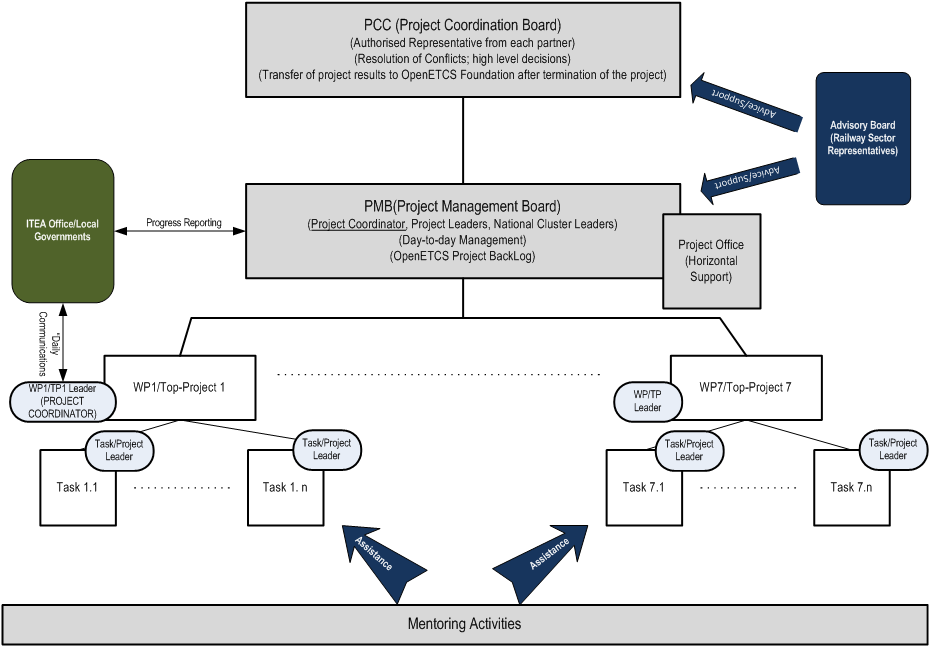
\includegraphics[scale=0.6]{./figures/project_structure.png}
\caption{OpenETCS Project Structure}
\end{figure}

\subsubsection{Compliance with ITEA Requirements}
ITEA rules are documented in the ITEA2 Frame Agreement [XX].

Compliance to ITEA Requirements is achieved by means of:
\begin{itemize}
\item The appointment of a Project Coordinator (DB, WP1, supported by the Project Office) who leads the project and is responsible for the communications with the ITEA representatives. 
\item The appointment of a Local Coordinator per country, National Cluster Leader, who reports to the corresponding National Authorities of the progress of the local partners
\item A signed PCA where cooperation rules and principles and working structures are agreed by all the partners.
\item An OpenETCS Foundation NV which guarantees sustainability of the project results once the project is finished.
\end{itemize}

\subsubsection{Compliance with Open Source Principles}
Compliance to the Open Source Principles and related objectives is achieved by means of:
\begin{itemize}
\item An OpenETCS IP Policy and Procedures \citep{IPP}
\item An OpenETCS Development Process \citep{odp} \href{https://github.com/openETCS/ecosystem/wiki/openETCS-Development-Process}{[Wiki]} based in the Eclipse Development Process \citep{EDP}, designed to promote dynamism in the development and openness. All the guidelines are maintained and available at the OpenETCS Ecosystem project [XX]: 
\begin{itemize}
\item The OpenETCS project is conceived as a project of projects organized in a hierarchical manner, where the WorkPackages, as defined within the WorkProgramme \citep{fpp}, are considered Top-Level Projects with their own charter. The so-called Tasks are projects, sub-projects of the corresponding Top-Level Project.
\item Anyhow, new projects can be launched, if needed and approved; existing projects can be archived, if they become inactive. Therefore the final structure of the OpenETCS project will very much depend on its evolution.  
\item The list of OpenETCS projects with information on their status is available in [XX]
\item Any project (independently to its position in the hierarchy, and type) has its project leader, scope and maintains its own resources. The project leader is not only responsible to guarantee progress towards the scope of the project but to promote that the most appropriate community is engaged in the project life-cycle with openness and transparency. This community includes committers, contributors, users and adopters.
\item Every Top-project/WP has its own repository under the responsibility of the Top-Project/WP Leader. Agreements and principles on the repository structure and content can be found in [XX] 
\item The PMB (Project Management Board) is responsible for maintaining and assuring the implementation of the OpenETCS Development Process and for ensuring the required “coordination” among the projects.
\item The Mentoring board (composed of XXX) is responsible for mentoring projects and advising.
\item The Project Office is responsible for the administrative tasks around the OpenETCS Development Process and maintains the OpenETCS Ecosystem project [XX]
\end{itemize}
\item The tools to support the OpenETCS Development Process are open source tools. A relation of the tools approved by the consortium is [XX]
\item The engagement of the OpenETCS Advisory Group will not only provide valuable technical insights but visibility of the project within the railway community.
\end{itemize}

\subsubsection{Compliance with SCRUM Requirements}
Agile Project Management ha been introduced to software projects in the 90-ties and is now a de-fact industry standard well documented in publications as e.g., in [XX].

Compliance to SCRUM Requirements is achieved by means of
\begin{itemize}
\item Each Work Package/Top-Project Leader is the SCRUM Product Owner of the corresponding WP/Top-Project results and maintains the corresponding backlog
\item Each Project/Task Leader is the SCRUM  Product Owner of the corresponding Tasks results  and maintains the corresponding backlog
\item The Project Coordinator is the SCRUM Product Owner of the project results and maintains the project results backlog.
\item Weekly meetings are maintained to find and report on impediments, assess progress, promote cross-collaboration, plan next steps and therefore, maintain the corresponding backlog.
\begin{itemize}
\item Weekly Scrum meetings are per definition open meetings, e.g., everybody from the teams can participate and contribute to the meeting.
\item The weekly meetings are strictly time-boxed.
\item At WP/Project level, the registered committers, contributors, users and adopters are invited to participate
\item At Open ETCS project level, the components of the PMB( Project Management Board) are invited.
\end{itemize} 
\item The work-packages resp. tasks need to organize there scrum teams according to practical needs.
\item Teams are typically distributed in geography and in organisation (i.e., participating companies).
\item Scrum teams typically have to provide several development roles (according to CENELEC and according to Eclipse). Guidance on the possible mixtrues of CENELEC roles into a Scrum team is documented in the annex section of this guideline.
\item To be able to be successful in Agile Development we need to set special focus to the role of the "User" of a product.
\begin{itemize}
\item In general, the user of a product in openETCS should representratives of the project openETCS consuming the result of a scrum team. 
\item The workpackage leader of the WP using an outcome of the team is the first candidate.
\item Representatives of partners making use of the openETCS result in long term are also natural users of a team result.
\item Partners in the openETCS project need to agree on the Users before the task when planning the interfaces. 
\end{itemize}  
\item Each team has to select a scrum master. Scrum training is mandatory.
\item A SCRUM master (WP1) is responsible for supporting the teams.
\end{itemize}

\subsubsection{Compliance with software management and organisation according to EN50128:2011}
In principle, two of the OpenETCS project results (Software and Tool Chain) are to be CENELEC SIL 4 certifiable. These are two of the results from WP3 and WP7. The following mechanisms, at organizational level, will help the corresponding project leader to provide evidence of compliance with chapters 5.1 \citep{EN50128} and 5.2. Anyhow, evidence that requirements imposed are met will have to be provided for each of the two software projects on a project by project basis. 

\begin{itemize}
\item Every partner in the consortium is ISO9001 Certified or will be in the position to provide evidence of a quality management process is accordance to ISO9001
\item Every partner maintains an updated CV of the staff/experts involved in OpenETCS
\item A Required Competence Matrix (RCM) per role and project will be maintained \textit{(Chapter 4)}.
\item A database with the participants per role and task/project will be maintained by the task/project leader.
\item Overall, the independence required to develop certifiable results is promoted by the Work Programme which is structured into the following “independent” WorkPackages/Top-Projects, each lead by a different organization.  
\begin{itemize}
\item WP2, focused on Requirements Specification is led by SNCF.
\item WP3, focused on the Software Implementation taking as input WP2 and WP7 results is led by Alstom France.
\item WP4 focused on the specification of the V\&V structure, is led by DLR
\item WP5 focused on demonstrating applicability/validity of WP3 and WP7 results is led by ERSA
\item WP7 focused on the development of the Tool Chain is led by DLR taking as input WP2 and WP4 inputs
\item For the purpose of validating/adapting technical approaches, tools and concepts before they are taken into consideration, three Use Cases will be engaged.
\item The Open Development Process facilitates the creation of the necessary projects required to achieve the OpenETCS project results.
\end{itemize}
\item For each assessable result, CENELEC required software roles will be covered by experts from different WPs. Incompatibilities can be controlled and monitored as active participation to the different projects has to be granted, accepted and is appropriately registered  \textit{(Chapter 2.2)}. Evidence of competence can be provided by comparing the CV of each expert with the RCM for the role assigned.
\item For each assessable result, if possible, the role of the assessor will be selected from the external community of the project. Meanwhile, an internal independent assessor will be appointed. The role and profile of this assessor is detailed in OpenETCS/internal-assessment \citep{IA} \href{https://github.com/openETCS/ecosystem/wiki/WP4:-internal-assessment}{[wiki pages]}
\end{itemize}

One of the mechanisms to guarantee the availability of competence staff when needed will be the design and implementation of a training programme. The training programme will be managed by the Project Office. The identification of needs will be performed by the project leaders, the PMB and the Quality Manager. 
The training process is detailed in [XX]


\subsection{Committers assignment and responsibilities}

Each Top-Project/WP leader is responsible for establishing and publishing the specific required competence matrix for the Top-Project/WP \textit{(Chapter 4)}. This matrix will be updated in response to the demands imposed by the evolution of the project. The competence matrix template \citep{Competence}is provided in [XX]

Each Top-Project/WP leader is responsible for developing the most appropriate communities of users, adopters, contributors and committers as required by the Top-Project/WP. A database will be maintained and assessed periodically by the Top-Project/WP Leader. This database will contain the coordinates of the expert, his/her role in the project and a basic explanation of adequacy. The expert database template is provided in [XX]

The required core competences as well as the expected contribution of each of the identified communities are described in Chapter 4.

Only committers have write-access to the project resources. Becoming a committer requires of the acceptance of the project leader and of the rest of the project committers. Guidelines on how to become a committer can be found in \href{https://github.com/openETCS/ecosystem/wiki/_pages}{[ecosystem wiki pages]}.

\begin{itemize}
\item It is the responsibility of the Project Leader to make sure the required competence to develop a task is covered by the engaged committers.
\item It is the responsibility of the Open ETCS Project Leader to guarantee the required competence for the project is covered by the effective committers.
\end{itemize}

Contributors have read-access to the project resources, and acceptance is not required. Guidelines on how to become a contributor can be found in \href{https://github.com/openETCS/ecosystem/wiki/_pages}{[ecosystem wiki pages]}.

An expert can contribute to different projects with different roles. The data from different project will be integrated and analysed to detect potential incompatibilities, if applicable. This activity will be done by the QA Manager. The guideline on how to select expert is detailed in [XX].


\subsection{Project QA Management}
QA activities will be under the responsibility of the QA Manager, who reports to the Project Coordinator.

The QA Manager will be responsible for the identification, supervision and control of all the processes, methods and tools required to meet the quality targets of the project. It is also the responsibility of the QA manager to provide the necessary evidence that such activities have been developed.

The activities of the QA Manager will be:
\begin{itemize}
\item To maintain the QA Plan and associated procedures and guidelines. 
\item A QA Plan Backlog will be maintained, implemented and published
\item To participate in the OpenETCS Ecosystem project in cooperation with the Project Office
\item To perform periodical audits of the maturity of the different on-going projects; propose improvement actions, if necessary.
\item To participate in the review processes of the different work products.
\item To collaborate with the Project Office in the identification of gaps and in the development of the corresponding Training Programme.
\item To perform quantitative and qualitative analysis at process and product levels. To maintain a set of metrics for all the processes.
\item To produce and publish the corresponding quality reports.
\end{itemize}


\newpage
\section{Life Cycle}

The openETCs project itself is a R\&D project running over 3 years which has the goal to deliver products such as the on-board specification model and the corresponding tool chain to generate source code based on this model. While the project life cycle is limited through the project time span, the products shall be used and also developed further after the end of the openETCS project. Respectively, the project only presents the firth development part of the product life cycle.

\subsection{Project Life Cycle }

The project Life Cycle is implemented through a set of WPs broken down into Tasks. In response of the nature of the project, these WPs are grouped into three purpose driven categories. The first category (WP2, WP4) addresses the specification of the work to be developed and the validation of the results to be obtained; the second category (WP3, WP7, WP5) addresses the development itself and the demonstration of the software and the tools chain developed and the third category (WP1, WP6) addresses the project management, the quality assurance and the dissemination of the project.
This structure permits both the development and the integration of conceptual (R\&D) and implementation activities to achieve innovative, validated and fit-for-purpose results.
The detailed description of the Work Package description and overview plan is covered by [FPP].  


\subsection{Product Life Cycle }

As the OpenETCS project products shall be part of the train development the reference for their life cycles are the CENELEC standard phases defined in the EN50126. But as the products are in general R\&D results, their life cycles do not include any certification or acceptance activities at the moment.
The main OpenETCS products are the OpenETCS Software model and the OpenETCS tools chain development, which have their own life cycles. For both parts the main development, verification and validation activities are done during the OpenETCS project. For the software only the demonstrator implementation is part of the OpenETCS project, while any kind of implementation on a target hardware is out of the project. 
For the OpenETCS tools chain the basic implementation is part of the project, but all further steps from qualification on are out of the project.
In general long time maintenance is a key concept of these products but it can not be established in the project time span. 

\subsubsection{Life Cycle of the OpenETCS Software}
The software development life-cycle of the OpenETCS project should be complied with CEN50128. Requirements imposed by the standard are analyzed and shown in detail in D2.2, while the software development life cycle applied in this project is described in Deliverable 2.3 and D2.4. The Test and Validation activities are presented in D4.2. The integration, the assessment and any maintenance is only defined in relation to the demonstrator implementation as no further phase can are planed in depth at this point.

\subsubsection{Life Cycle of the OpenETCS Tools chain}
The development of the Tool Chain has to comply with EN50128. Requirements imposed by the standard are analyzed and shown in detail in D2.2. The tools chain development life cycle is described in D7.3. As the tools chain is a combination and improvement of already existing tools, which have a specific life-cycle, the tools chain life cycle mainly consists of integration and maintenance activities. 

\subsection{QA Management }
\textit{Guidance: Refer to the procedures to implement the QA activities identified within the above mentioned development life-cycle. }

\todo[color=yellow!20, inline]{CC: The parts §2.3 (Project QA management) and 3.3 (QA management) could be both in the same part (2 or 3). For us, the Quality Assurance has to refer to both project life-cycle and Software life-cycle.}

\todo[color=green!20, inline]{IT: In chapter 2.2, the idea is to introduce the QA Organisation Roles (both project and software, as you say).
In chapter 3.3 we will explain the QA activities}

\section{Roles}

\newcommand\todoin[2][]{\todo[inline, caption={2do}, #1]{
\begin{minipage}{\textwidth-4pt}#2\end{minipage}}}

\subsection{OpenETCS Roles}

In view of the nature of the project, roles are grouped into three independent categories:

\begin{itemize}
\item CAT1: Open Source Development Process Roles
\item CAT2: SCRUM Roles
\item CAT3: CENELEC Roles 
\end{itemize}

Therefore, any participant will always adopt a role within CAT1, a role within CAT2 and if he/she is involved in the development of a CENELEC assessable product, a third role in CAT3.

As already mentioned, OpenETCS is a project of projects. An expert can participate to different projects with different roles. Therefore an expert will have a CAT1, CAT2 and/or CAT3 role per project.

In the Annexes A, B, C and D, the responsibilities and the core competences required by each role are detailed. It is the responsibility of the QA Manager to keep them updated

In the case of CAT 1 roles, specific technical competence will be required depending on the scope of the project. For this reason a new column has been added. In this column, specific technical competences for each project and role are to be included. It is the responsibility of each project leader to provide this information.

According to the open development process followed by Open ETCS, the QA process is also a project. For this reason the QA Manager will have to meet the competences of a Project Leader and the specific competences imposed by CENELEC and the OpenETCS project to the Quality Manager activities. When needed, specific responsibilities imposed by a project to a role will be detailed too.

As project results affected by CENELEC are already identified, both core and specific required competence per CAT 3 role are included in Annexes C and D.

\subsection{Roles within the Development process of the openETCS Software}
The responsibilities and competences for every role specific to the openETCS Software development are listed in Annex C. The independence of different roles is the core concept of the quality assurance strategy required be CENELEC standards. As openETCS is a collective project by various independent partners, the project organization already ensures full independence between the roles administrated by experts from different partners. 

\subsection{Roles within the Development process of the openETCS Tools Chain}

See Annex D
\subsection{QA Activities}

The QA Manager will be in charge of:
\begin{itemize}
\item Maintaining the Requirements Competence Matrices updated in response to the evolution of the OpenETCS project
\item Performing periodical audits of the participants{\textquotesingle} database per project; trace database with the RCM (Required Competence Matrix) for such project
\item Identify training needs and provide the required support to the Project Office in the definition and organization of the corresponding training activities.
\item In the case of CENELEC related project, provide the necessary evidence of competence and independency between roles. If this is not possible, propose the necessary solutions and support the projects in its implementation
\end{itemize}

\section{Methods, measures and tools for quality assurance (product + open ETCS software + Tools chain)}


Selection of methods and tools used in each phase of the OpenETCS process is a part of the WP7 activities. This selection is based on the state of art established by WP2 (D2.1 and D2.2), the set of requirements defined by WP2 (D2.6-9) and the process definition (D2.3, D2.4, D4.1, D4.2.3).

Results of the selection of methods and tools are given in the D7.1 and D7.2 deliverables. Conformance of the methods and tools are going to be discussed in D7.3.

The following table give details of all this deliverables.

\begin{table}[H]
\begin{supertabular}{|m{3cm}|m{11cm}|}
\hline
\rowcolor{myblue}
Deliverable &
Content of Relevance for this Chapter\\\hline
D2.1: Report on existing methodologies &
State of the art on methods and tools \\\hline
D2.2: Report on CENELEC Standards &
CENELEC requirements to be fulfilled and the approach followed by the project to provide evidence\\\hline
D2.3: Process definition &
OpenETCS process definition \\\hline
D2.4: Report on Methods definition &
Description of methods and tools to use to follow the OpenETCS process \\\hline
D2.6-9: Set of requirements for the OpenETCS project &
Definition of the requirements that the selected methods and tools shall follow \\\hline
D4.1: Report on V\&V Plan \& Methodology &
Detailed description of the V\&V process and how are used the methods and tools to cover V\&V artifacts \\\hline
D4.2.3: Safety Plan &
Detailed requirements on methods and tools to be used during the process to obtain a SIL4 developement of on-board unit \\\hline
D7.1: Report on the final choice(s) for the primary tool chain (means of description, tool and platform) &
Selected methods and tools to be used during the specification and design part of the OpenETCS process \\\hline
D7.2: Report on all aspects of secondary tooling (results of T7.2)  &
Selected methods and tools to complete the OpenETCS process (V\&V, safety analyses,..) \\\hline
D7.3: Tool chain qualification process description &
This report describe how the selected methods and tools fit the qualification requirements according CENELEC standard \\\hline
\end{supertabular}
\caption{Referenced deliverables}
\end{table}


\subsection{Methods, measures and tools for quality assurance OpenETCS Application Software}

It is assumed that the OpenETCS application software will be SIL4 compliant. Therefore, the methods, techniques and tools shall be suitable to SIL 4. 


\todo[color=yellow!20, inline]{MPD(Systerel): It is not totally exact: one of the aim of the project is to provide a tool chain which allows to develop SIL4 software, the OpenETCS applcation software produced during the project has not as objective to be SIL4 compliant.}


\todo[color=yellow!20, inline]{MPD(Systerel): The current OpenETCS process, and the selection of methods and tools, do not cover only software development but also system phases as described in EN50129 or EN50126.}

\subsection{Methods, measures and tools for quality assurance openETCS Tools chain}

The Tool Chain will be composed of a set of tools with different levels of interaction. The document D7.3 provides a description of the Tool Chain architecture, jointly with a description of the constituent tools.
Following CENELEC criteria, each tool belongs to one of the following classes: T1, T2 and T3. Class 3 and Class 2 Tools are obliged to follow specific development methods, techniques and tools. 


\subsection{Quality Control and Monitoring Activities}
\textit{Guidance: Describe the measures to monitor the appropriate implementation of the selected methods and tools.}

\todo[color=yellow!20, inline]{JW: This is a broad topic, the main issues will be covered by the verification, validation and safety plan. This aspect should introduce the general principals and tools and then reference those documents.}

\todo[color=green!20, inline]{IT: OK. I think there is an error in the template. Instead of QA Activities, it is Quality Control and Monitoring Activities.}

\section{Documentation}

The documentation structure of the OpenETCS project is composed of:
\begin{itemize}
\item Deliverables, which constitute the official outcomes of the different Top-Projects/WPs
\begin{itemize}
\item The relation and scope of the deliverables to be produced along OpenETCS can be found in the FPP [].
\item The updated status of development of each Deliverable can be found in 
\href{https://github.com/openETCS/management/wiki/State-of-Deliverables}{[State-of-Deliverables Wiki]}.
\item The approved and therefore valid version of each Deliverables can be found in the repository of the Top-Project/WP it belongs to. 
\end{itemize}
\item Contractual documents, with the Commission and among the project partners
\begin{itemize}
\item The status of development of each contractual document can be found under the repository of Management (WP1).
\item The last approved and therefore valid version of each contractual document can be found under the repository of Management (WP1).
\end{itemize}
\item Periodic Progress Reports, to show progress to ITEA and EC representatives.
\begin{itemize}
\item The state of each Periodic Report can be found under repository of Management (WP1).
\item The last approved and therefore valid version of each Periodic Progress Report can be found under the repository of Management (WP1). 
\end{itemize}
\item Supporting Documents, in the form of Templates and Procedures
\begin{itemize}
\item The procedures and templates applicable to a specific Top-Project/WP can be found in the repository of the corresponding TP/WP.
\item The procedures and templates applicable to the whole project can be found in the repository of Governance.
\end{itemize}
\item Internal Reports, in the form of Meeting Minutes
\begin{itemize}
\item The minutes of the weekly scrum meetings are found in the repository of Governance.
\end{itemize}
\end{itemize}

The nomenclature used for the naming of the different documents is provided in [XX-to be developed].

For each TP/WP the relation of existing documents is provided in the form of a list \href{https://github.com/openETCS/governance/wiki}{[Wiki]}. This list includes a direct access to the valid version of each document.

\subsection{Documentation Structure within the development process of the openETCS Software}
As a SIL4 software, the documentation structure has to comply with CENELEC requirements. The following table shows the document structure required by CENELEC for a SIL4 development and the corresponding documents produced in the OpenETCS project.

\begin{center}
\begin{longtable}{|m{2cm}|m{1cm}|m{7cm}|m{2cm}|m{2cm}|}
\caption{Documentation Structure}\\

\hline \rowcolor{myblue} \multicolumn{5}{|c|}{\textbf{Documentation Structure within the development process of the openETCS Software}} \\ \rowcolor{lightgray} \multicolumn{1}{|c|}{\textbf{Phase}} & \multicolumn{1}{c|}{\textbf{SIL4}} & \multicolumn{1}{c|}{\textbf{Document}} & \multicolumn{1}{c|}{\textbf{WP/Task}} & \multicolumn{1}{c|}{\textbf{Link}} \\ \hline 
\endfirsthead

\multicolumn{5}{c}%
{{\bfseries \tablename\ \thetable{} -- continued from previous page}} \\
\rowcolor{myblue} \multicolumn{5}{|c|}{\textbf{Documentation Structure within the development process of the openETCS Software}} \\
\rowcolor{lightgray} \multicolumn{1}{|c|}{\textbf{Phase}} & \multicolumn{1}{c|}{\textbf{SIL4}} & \multicolumn{1}{c|}{\textbf{Document}} & \multicolumn{1}{c|}{\textbf{WP/Task}} & \multicolumn{1}{c|}{\textbf{Link}} \\ \hline 
\endhead

\hline \multicolumn{5}{|r|}{{Continued on next page}} \\ \hline
\endfoot

\hline \hline
\endlastfoot

Planning &
\centering HR &
\raggedright
Software Quality Assurance Plan\\
Software Quality Assurance Verification Report\\
Software Configuration Management Plan\\
Software Verification and Validation Plan\\ &
(to be defined) &
(to be defined)
\\\hline
Software Requirements &
\centering HR &
\raggedright
Software Requirements Specification\\
Software Requirements Test Specification\\
Software Requirements Verification Report\\ &
(to be defined) &
(to be defined)
\\\hline
Architecture and design &
\centering HR &
\raggedright
Software Architecture Specification\\
Software Design Specification\\
Software Interface Specification\\ 
Software Integration Test Specification\\ 
Software/Hardware Integration Test Specification\\ 
Software Architecture and design verification report\\ &
(to be defined) &
(to be defined)
\\\hline
Component Design &
\centering HR &
\raggedright
Software Component design specification\\
Software Component Test Specification\\
Software Component design verification report\\ &
(to be defined) &
(to be defined)
\\\hline
Component Implementation and Testing &
\centering HR &
\raggedright
Software source code and supporting documentation\\
Software source code verification report\\
Software Component Test Report\\ &
(to be defined) &
(to be defined)
\\\hline
Integration &
\centering HR &
\raggedright
Software Integration Test Report\\
Software/Hardware Integration Test Report\\
Software Integration Verification Report\\ &
(to be defined) &
(to be defined)
\\\hline
Overall Software Testing/Final validation &
\centering HR &
\raggedright
Overall Software Test Report\\
Software Validation Report\\
Tools Validation Report\\ 
Release Note\\ &
(to be defined) &
(to be defined)
\\\hline
Systems configured by Application Data/algorithms &
\centering HR &
\raggedright
Application Requirements Specification\\
Application Preparation Plan\\
Application Test Specification\\ 
Application Architecture and Design\\ 
Application Preparation Verification Report\\ 
Application Test Report\\ 
Source Code of Application Data/Algorithms\\ 
Application Data/Algorithms Verification Report\\ &
(to be defined) &
(to be defined)
\\\hline
Software Deployment &
\centering HR &
\raggedright
Software Release and Deployment Plan\\
Software Deployment Manual\\
Release Notes\\ 
Deployment Records\\ 
Deployment Verification Report\\ &
(to be defined) &
(to be defined)
\\\hline
Software Maintenance &
\centering HR &
\raggedright
Software Maintenance Plan\\
Software Change Records\\
Software Maintenance Records\\ 
Software Maintenance Verification Report\\ &
(to be defined) &
(to be defined)
\\\hline
Software Assessment &
\centering HR &
\raggedright
Software Assessment Plan\\ 
Software Assessment Report\\ &
(to be defined) &
(to be defined)
\\\hline
\end{longtable}
\end{center}


\subsection{Documentation Structure within the development process of the openETCS Tools chain}
\textit{Guidance: See Chapter 6.1}


\subsection{Quality Control and Monitoring Activities}
\textit{Guidance: Describe the methods to review the documentation structure}

\todo[color=yellow!20, inline]{JW: For me this should not be the review of the documentation structure, but the documentation quality control activities. These are looked at in detail over the next to chapters, therefore this should be a general overview.}

\todo[color=green!20, inline]{IT: OK}

\section{Documentation Control}
\textit{Guidance: Refer to Control Process Document where the function develop by authors, reviewers is provider}

\todo[color=yellow!20, inline]{JW: This sentence is hard to understand. From my point of view the three section make no sense since there should be the same process for all kinds of documents. This section should name the main control activities (review, approval, dissemination, archiving) and the main tools used for this. Then it should refer do the respective documents (like the great review process).}
\todo[color=green!20, inline]{IT: OK, we will clarify this sentence.}

\subsection{Documentation Control within the Development process of the openETCS Sotware}
\textit{Guidance: Refer to the list of active documents of the openETCS software}

\subsection{Documentation Control within the Development process of the openETCS Tools chain}
\textit{Guidance: Refer to the list of active documents of the openETCS tools chain}

\subsection{Quality Control and Monitoring Activities}
\textit{Guidance: Describe the methods to monitor both the control and process}

\section{Tracking and tracing of deviation}


\subsection{Traceability (openETCS software + Tools chain)}
\textit{Guidance: Provide a description of traceability requirements, as well as how the traceability will be achieved, implement, maintained and verified. At this stage, exceptions if they exist should be justified.}

\subsection{Configuration Management}
\textit{Guidance: Refer to SCMP (System Configuration Management Plan). Overview table with the summary of main features of SCMP.}

\todo[color=yellow!20, inline]{JW: SCMP has to be written. This mainly includes an explanation of the proper github working processes.}
\todo[color=green!20, inline]{IT: OK, it will be included in the backlog we are preparing.}

\textit{Describe the QA activities}

\subsection{Fault Management}

ISTQB define a defect as "a flaw in a component or system that can cause the component or system to fail to perform its required function". A defect can be random or systematic. A defect, if encountered during execution, may cause a failure of the component or system". From the ISTQ glossary bug, fault and problem are defined to be the same as a defect.

A failure is a deviation of the component or system from its expected delivery, service or result. A failure is the consequence of a fault or error in a system but not all faults result in failures.

Faults, failures and errors encountered during the review activities (QA. Verification, Validation, Assessment) planned in the software development life-cycle, problems reported by users and customers as well as change requests initiated by any of the system stakeholders will be reported and managed following the Change/Problem Management Process  \citep{emp} detailed in [XX] and through the Change/Problem Management Tool. This tool will be integrated with the Configuration management tool {\it GIT} and will be configured to implement and record all the information generated during the process.

The integration with the Configuration management tool {\it GIT} will permit:
\begin{itemize}
\item Traceability between Change/Problem Requests and the configuration items where the problem was located.
\item Traceability between the configuration items modified and the corresponding Change/problem request. 
\end{itemize}
 
The implementation of the workflow will permit:
\begin{itemize}
\item A complete history trail of the Change Request/Problem Report
\end{itemize}

The purpose of the Change/Problems Management implementation at OpenETCS project is to ensure that standardized methods and procedures are used for efficient and prompt handling of all changes/problems associated with the OpenETCS products, in order to minimize the number and impact of any related changes/problems. Changes/problems in the products may arise reactively in response to incidents, or proactively from seeking improved efficiency and effectiveness, as well as to enable or reflect OpenETCS initiatives, or products improvements.

The QA Manager will be in charge of:
\begin{itemize}
\item perform periodical audits and quality assessments of the bugs received
\begin{itemize}
\item Audits to verify the process itself
\item Quality Assessments to verify the evolution of the product quality
\end{itemize}
\item Assist in determining QA impacts
\item Support Problem owner in analysis
\end{itemize}

\subsection{Grievance Handling}
\textit{Guidance: Refer to the specific procedure. }

\textit{Describe the QA activities}

\subsection{Modification and change control }

A change is the addition, modification, or removal of a configuration item (CI), product, or product component, and/or its associated elements

The change requests initiated by any of the system stakeholders will be reported and managed following the Change/Problem Management Process  \citep{emp} detailed in \href{https://github.com/openETCS/governance/tree/master/Change-Problem%20Process}{[governance]} and through the Change/Problem Management Tool.

The Change/problem Management process aims to evaluate and plan the change/problem process to ensure that, if a change is made, it is done in the most efficient way possible, following the established procedures and ensuring the quality and continuity of the OpenETCS project and products at all times.

The QA Manager will be in charge of:
\begin{itemize}
\item perform periodical audits and quality assessments of the change request received
\begin{itemize}
\item Audits to verify the process itself
\item Quality Assessments to verify the evolution of the product quality
\end{itemize}
\item Assist in determining QA impacts
\item Support Change owner in analysis
\end{itemize}


\section{Supplier Control}
\textit{Guidance: Requirements to external suppliers and how they will be verified}

\todo[color=yellow!20, inline]{JW: What are the suppliers in OpenETCs and what activities are needed here?}
\todo[color=green!20, inline]{IT: It is only to be considered if any supplier is needed}

\textit{describe the QA activities to be developed.}

\todo[color=yellow!20, inline]{JW: Im missing sections for the Quality Assurance during the product maintenance and the deployment of the software and the tool chain.}
\todo[color=green!20, inline]{IT: Product Maintenance and deployment phased will be covered in Chapter 3.2}

\newpage
\begin{landscape}
\section{ANNEXES}

\subsection{ANNEX A -CAT1: Open Source Development Process Roles and Competence Matrix-}

\begin{center}
\begin{longtable}{|m{1cm}|m{2,20cm}|m{8,70cm}|m{4,6cm}|m{4,6cm}|}
\caption{CAT1: Open Source Development Process Roles/Competences}\\

\hline \rowcolor{myblue} \multicolumn{5}{|c|}{CAT1: Open Source Development Process Roles/Competences} \\ \rowcolor{lightgray} \multicolumn{1}{|c|}{Code} & \multicolumn{1}{|c|}{Role} & \multicolumn{1}{|c|}{Responsibilities (To be revised)} & \multicolumn{1}{|c|}{Core Competences} & \multicolumn{0}{|c|}{Specific Competences
 /Responsibilities per project} \\ \hline 
\endfirsthead

\multicolumn{5}{c}%
{{\bfseries \tablename\ \thetable{} -- continued from previous page}} \\
\hline \rowcolor{myblue} \multicolumn{5}{|c|}{CAT1: Open Source Development Process Roles/Competences} \\ \rowcolor{lightgray} \multicolumn{1}{|c|}{Code} & \multicolumn{1}{|c|}{Role} & \multicolumn{1}{|c|}{Responsibilities (To be revised)} & \multicolumn{1}{|c|}{Core Competences} & \multicolumn{0}{|c|}{Specific Competences
 /Responsibilities per project} \\ \hline
\endhead

\hline \multicolumn{5}{|r|}{{Continued on next page}} \\ \hline
\endfoot

\hline \hline
\endlastfoot

OPL &
OpenETCS project Leader &
\raggedright
Responsible to guarantee progress\\
Promote that the most appropriate community is engaged in the project life-cycle\\
Ensure that all personnel involved in all phases of the software, tool chain (products)  and project life-cycle, including management activities, have the appropriate training, experience and qualifications
&
\textbf{(To be fulfilled)} &
\textbf{(To be fulfilled per project)} \\\hline
WPL &
WP Leader/Top-level project leader &
\raggedright
Make sure the required competence to develop a task is covered by the engaged committers\\
To ensure that all personnel who have responsibilities for the software are competent to discharge those responsibilities\\
Ensure that the parties involved throughout the product life-cycle are independent, to the extent required by the software safety integrity level, in accordance with cenelec
&
\textbf{(To be fulfilled)} &
\textbf{(To be fulfilled per project)} \\\hline
TL &
Task Leader/ project leader &
\raggedright
Maintains the corresponding backlog\\
&
\textbf{(To be fulfilled)} &
\textbf{(To be fulfilled per project)}\
Project: QA activities
\begin{description}
\item responsible for the identification, supervision and control of all the processes, methods and tools required to meet the quality targets of the project
\end{description}
\\\hline
US &
User &
\raggedright
Not Applicable &
\textbf{(To be fulfilled)} &
\textbf{(To be fulfilled per project)} \\\hline
AD &
Adopter &
\raggedright
Reuse of the frameworks (within the companies that are contributing to the project and outside of the project),\\
Reuse of the tools (within the companies that are contributing to the project and outside of the project,
&
\textbf{(To be fulfilled)} &
\textbf{(To be fulfilled per project)} \\\hline
CTB &
Contributor &
\raggedright
Contribute content, code, fixes, tests, documentation, or other work that is part of the Project\\
Provide feedback\\
Help new users\\
Test, report or fix bugs\\
Request new features\\
Write or update documentation\\
Write and update software
&
\textbf{(To be fulfilled)} &
\textbf{(To be fulfilled per project)} \\\hline
CMT &
Committer &
\raggedright
Have the exclusive right to elect new Committers to their Project–no other group, including a parent Project, can force a Project to accept a new Committer.\\
Monitor and contribute to the mailing lists\\
Proactively report problems in the task tracking system, and annotating problem reports with status information, explanations, clarifications, or requests for more information from the submitter
&
\textbf{(To be fulfilled)} &
\textbf{(To be fulfilled per project)} \\\hline
\end{longtable}
\end{center}


\newpage
\subsection{ANNEX B -CAT2: SCRUM Roles and Competence Matrix-}

\begin{center}
\begin{longtable}{|m{1cm}|m{4cm}|m{12cm}|m{7,5cm}|}
\caption{CAT2: SCRUM Roles/Competences}\\

\hline \rowcolor{myblue} \multicolumn{4}{|c|}{CAT2: SCRUM Roles/Competences} \\ \rowcolor{lightgray} \multicolumn{1}{|c|}{Code} & \multicolumn{1}{|c|}{Role} & \multicolumn{1}{|c|}{Responsibilities \textbf{(To be revised)}} & \multicolumn{1}{|c|}{Core Competences} \\ \hline 
\endfirsthead

\multicolumn{4}{c}%
{{\bfseries \tablename\ \thetable{} -- continued from previous page}} \\
\hline \rowcolor{myblue} \multicolumn{4}{|c|}{CAT2: SCRUM Roles/Competences} \\ \rowcolor{lightgray} \multicolumn{1}{|c|}{Code} & \multicolumn{1}{|c|}{Role} & \multicolumn{1}{|c|}{Responsibilities \textbf{(To be revised)}} & \multicolumn{1}{|c|}{Core Competences} \\ \hline
\endhead

\hline \multicolumn{4}{|r|}{{Continued on next page}} \\ \hline
\endfoot

\hline \hline
\endlastfoot

POw &
Product Owner &
\raggedright
Managing and prioritizing the Product Backlog\\
Planning the release\\
Software and Tool chain acceptance\\
Understand the value of the project
&
\textbf{(To be fulfilled)} \\\hline
ScM &
Scrum Master &
\raggedright
Planning the Sprints\\
Prioritizing the sprint backlog\\
Team leader\\
Manage the development process \\
Prepare Burndown charts\\
Identify and eliminate obstacles that prevent the team from achieving their goals \\
Ensures that the team is fully functional and productive\\
Enables close cooperation across all roles and functions\\
Ensure clear communication among everyone involved in the project
&
\textbf{(To be fulfilled)} \\\hline
ScT &
Scrum Team &
\raggedright
Self organizing (organizes itself and its work)\\
Identify obstacles and informing the Scrum Master \\
Development to achieve sprint goals.\\ 
Implementing test cases \\
Unit and initial Acceptance testing 
&
\textbf{(To be fulfilled)} \\\hline
\end{longtable}
\end{center}

\newpage
\subsection{ANNEX C -CAT3: CENELEC Roles and Competence Matrix for OpenETCS software product-}

\begin{center}
\begin{longtable}{|m{1cm}|m{2,5cm}|m{11cm}|m{10cm}|}
\caption{CAT3: CENELEC Roles/Competences for OpenETCS application software project}\\

\hline \rowcolor{myblue} \multicolumn{4}{|c|}{CAT3: CENELEC Roles/Competences for OpenETCS application software project} \\ \rowcolor{lightgray} \multicolumn{1}{|c|}{Code} & \multicolumn{1}{|c|}{Role} & \multicolumn{1}{|c|}{Responsibilities \textbf{(To be revised)}} & \multicolumn{1}{|c|}{Competences} \\ \hline 
\endfirsthead

\multicolumn{4}{c}%
{{\bfseries \tablename\ \thetable{} -- continued from previous page}} \\
\hline \rowcolor{myblue} \multicolumn{4}{|c|}{CAT3: CENELEC Roles/Competences for OpenETCS application software project} \\ \rowcolor{lightgray} \multicolumn{1}{|c|}{Code} & \multicolumn{1}{|c|}{Role} & \multicolumn{1}{|c|}{Responsibilities \textbf{(To be revised)}} & \multicolumn{1}{|c|}{Competences} \\ \hline 
\endhead

\hline \multicolumn{4}{|r|}{{Continued on next page}} \\ \hline
\endfoot

\hline \hline
\endlastfoot

PM &
OpenETCS software Project Manager &
\parbox{11cm}{\raggedright
Identify which roles are needed for the project\\
Verify that at least one person fulfills an identified project role\\
Guarantee the required competence for the project is covered by the effective committers\\
Initialize the distribution of roles between partners to ensure independence of the roles\\
Ensure compliance with the quality management system\\
Responsible to guarantee progress according to scheduled plans\\
Responsible for the delivery and implementation of the software\\
Ensure the compliance and the delivery of safety requirements\\
Approve full and partial products to be delivered by the development process\\
Ensure that records and traceability are maintained throughout the decision making and project\\
Ensure appropriate validation for the project through project partners}
&
\parbox{10cm}{\raggedright
Understand requirements of software development process\\
Understand quality, competencies, organizational and management requirements according to relevant standards\\
Understand the requirements of the verification, validation and safety process\\
Able to evaluated the impact of different options for the performance concerning implementation, validation and safety}
\\\hline
RQM &
Requirement manager &
\parbox{11cm}{\raggedright
Responsible for the software model and source code requirement specification\\
Establishes and maintain traceability to and from the system-level requirements\\
Ensure that software and derived specifications requirements are under system\\ configuration and changes management control.\\
Ensure consistency and completeness of the software requirements specification\\
Develop and maintain documents related to software requirements
}&
\parbox{10cm}{\raggedright
experience in railways sector and safety attributes in the railway domain\\
experience with requirements management process and tools\\
knowledges of TSI and related CENELEC requirements}
\\\hline
DES &
Designer &
\parbox{11cm}{\raggedright
Transform software requirements on acceptable solutions\\
Derive the requirements for the system and software architecture\\
Identify the key design issues that must be resolved to support successful development of the software\\
Allocate the software and derived requirements to the chosen architecture components and interfaces\\
Maintain requirement traceability for the software architecture{\textquotesingle}s requirements, and to and from software requirements\\
Identify suitable derived requirements that address the effectiveness and cost of life-cycle phases following development, such as production and operation\\
Develop and maintain design documentation\\
Ensure that the design documents are under system configuration and changes management control.\\
Design or select design methods and support tools\\
Apply principles and suitable design standards\\
Develop component specifications if it is applicable
}&
\parbox{10cm}{\raggedright
Competent in software development in the railway domain\\
Competent in safety design principles\\
Familiarity with methods and tools for design analysis and design testing\\
Ability to work with design constraints for safety relevant software in On-Board systems\\
Understanding of the system constraints created through the TSI\\
Understanding of the relevant parts of EN 50128 like design methods}
\\\hline
IMP &
Implementer &
\parbox{11cm}{\raggedright
Transform design solutions in data, models, source code and finally executable code for the demonstrator\\
Apply safety design principles\\
Apply specific rules for data preparation/codification\\
Perform analysis to verify intermediate results\\
Develop and maintain implementing documents comprising the methods, types of data, models and listings applied\\
Maintain traceability to and from the design\\
Maintain the generated or modified data/codes/models under system configuration and changes management control.
}&
\parbox{10cm}{\raggedright
Competent in safety relevant software implementation for embedded systems\\
Competent in the implementation language and supporting tools\\
Capable of applying the specified coding standards and programming styles\\
Understanding of the system constraints created through the On-Board hardware respectively the demonstrator\\
Understanding of the relevant parts of EN 50128 like design methods}
\\\hline
TST &
Tester &
\parbox{11cm}{\raggedright
Ensure the test activities planning \\
Develop tests specification (goals and cases)\\
Ensure traceability of test objectives to specified software requirements\\
Ensure traceability of test cases to the specified tests objectives\\
Ensure that the planned tests are implemented and performed\\
Identify deviations from the expected results and record in the test reports\\
Communicate deviation to the authority in charge of the changes management for evaluation and decision making\\
Record the results reports\\
Select the equipment for testing the software
}&
\parbox{10cm}{\raggedright
Competent in ETCS specification, used means of description (model/ source code), used train and track parameter and other application data source\\
Competent in various test approaches/methods to identify to identify the most appropriate method or combination of methods for every aspect of an artifact\\
Capable of deriving test cases from TSI (specifically Subset 26) and the specification model\\
Understanding of the relevant parts of EN 50128 like test methods}
\\\hline
VER &
Verifier &
\parbox{11cm}{\raggedright
Develop a SW Verification Plan \\
Check the documented test suitability (completeness, coherency, relevance, traceability) with the verification objectives\\
Identify anomalies, evaluate in terms of the risk, record them and communicate them to the authority in charge of the changes management for evaluation and decision making\\
Manage the verification process (revision, integration and testing) and ensure the independence of the activities as needed\\
Develop a verification report with the results of the verification activities
} &
\parbox{10cm}{\raggedright
Competent in ETCS specification, used means of description (model/ source code), used train and track parameter and other application data source\\
Competent in various verification approaches/methods to identify the most appropriate method or combination of methods for every aspect of an artifact\\
Capable of deriving verification procedures from TSI (specifically Subset 26) and the specification model\\
Understanding of the relevant parts of EN 50128 like verification methods}
\\\hline
INT &
Integrator &
\parbox{11cm}{\raggedright
Manage the integration process using software baselines\\
Develop sw and sw /hw integration test specification for sw components based on the specifications and on the designer{\textquotesingle}s components architecture \\
Develop and maintain records of the integration activities\\
Identify integration anomalies; record them and communicate them to the authority in charge of the changes management for evaluation and decision making\\
Develop a report of components and the overall system integration covering the integration results 
}&
\parbox{10cm}{\raggedright
Competent in ETCS specification, used programming language, used API and demonstrator hardware\\
Competent in various integration approaches/methods to identify the most appropriate method or combination of methods for the demonstrator implementation\\
Understanding the design and functionality requirements for intermediated development levels\\
Capable of deriving integrator tests from the set of integrated functions\\
Understanding of the relevant parts of EN 50128 like integration tests}
\\\hline
VAL &
Validator &
\parbox{11cm}{\raggedright
Develop a Validation Plan specifying the main tasks and activities for the sw validation\\
Agree on the Validation Plan with the assessor\\
Review Sw requirements in relation to their intended use/environment\\
Ensure sw fulfill all sw requirements\\
Evaluate the assessment of the software process and of the software according to CENELEC requirements and the assigned SIL\\
Review the verification and tests correctness, consistency and suitability \\
Check the correctness, consistency and suitability of the test cases and executed tests\\
Ensure that all validation plan activities are carried out\\
Review and classify deviations, evaluate in terms of the risk, record them and communicate them to the authority in charge of the changes management for evaluation and decision making\\ 
Provide recommendation about sw suitability\\
Record Validation Plan deviations\\
Conduct audits, inspections or reviews of the overall project at various stages of development as may be appropriate\\
Review and analyse validation reports of the previous sw\\
Check whether the developed solutions are traceable to the sw requirements \\
Ensure that records associated hazardous situations and nonconformances are reviewed\\
Ensure that all dangerous situations are appropriately resolved\\
Develop a Validation Report\\
Express their agreement or disagreement about the sw version  
}&
\parbox{10cm}{\raggedright
Competent in ETCS On-Board units\\
Experience in safety attributes for train control systems\\
Competent in various validation approaches/methods to identify the most appropriate method or combination of methods for the demonstrator implementation\\
Capable of deriving types of validation evidence required for the TSI with respect to the train control functionality\\
Capable to combine different sources and types of evidence and synthesize an overall view about fitness for purpose or constraints and limitations of the On-Board application\\
Overall software understanding and perspective including the general railway environment\\
Understanding the requirements of EN 50128}
\\\hline
ASR &
Assessor &
\parbox{11cm}{\raggedright
Develop an assessment plan and communication with safety authority and client organization\\
Evaluate the assessment of the software process and of the software according to CENELEC requirements and the assigned SIL\\
Assess the project team and the organization competences for the sw development\\
Evaluate the Verification \& Validation activities and the supporting evidences\\
Evaluate quality management systems adopted for  the sw development\\
Evaluate the changes management and the Configuration Management Systems and their use\\
Identify and assess risk in terms of any deviation from the sw requirements in the evaluation report\\
Ensure the evaluation Plan is implemented\\
Performs independent checks of: The development process (audits) and the products safety functions (spot checks) during different development phases.\\
Should perform audits, based on the Safety plan, of the Quality and Safety management systems of the Supplier, the Infrastructure owner and the Operator and be convinced that these systems works\\
The Assessor can also perform spot checks on detailed technical issues to see that safety functions are correctly implemented. The safety functions key documentation (Hazard Log, Safety Requirements and Safety Case) should be examined too.\\
Give an opinion on the validity of sw developed for its intended use detailing any constraints, application conditions and observations for risk control appropriate\\
Develop an assessment report and maintain records about the assessment process
}&
\parbox{10cm}{\raggedright
Competences in the railway domain and technology specifically concerning On-Board systems\\
Acceptance/License from a recognized safety authority\\
Continually gained sufficient level of experience in the safety principles and the application of these principles within the railway domain\\
Competence to evaluated that a suitable method or combination of methods in a given context have been applied\\
Understanding the relevant safety, human resource, technical and quality management processes to fulfill the requirements of the EN 50128\\
Competence in assessment approaches/ methods\\
Capable to combine different sources and types of evidence and synthesize an overall view about fitness for purpose or constraints and limitations of the On-Board application\\
Overall software understanding and perspective including the general railway environment\\
Ability to judge the adequacy of all development processes (like quality management, configuration management, validation and verification processes)\\
Understanding the requirements of EN 50128}
\\\hline
CM &
Configuration Manager &
\parbox{11cm}{\raggedright
Responsible for the configuration management plan \citep{scmp}
System configuration management owner\\
Establish that all sw components are clearly identified and have independent versions within the system configuration management\\
Prepare the published release notes mentioning incompatible versions of sw components
}&
\parbox{10cm}{\raggedright
Competences in software configuration management\\
Understanding the requirements of EN 50128}
\\\hline
\end{longtable}
\end{center}

\newpage


\subsection{ANNEX D -CAT3: CENELEC Roles and Competence Matrix for OpenETCS Tool Chain product-}

\begin{center}
\begin{longtable}{|m{1cm}|m{2,5cm}|m{11cm}|m{10cm}|}
\caption{CAT3: CENELEC Roles/Competences for OpenETCS Tool Chain product}\\

\hline \rowcolor{myblue} \multicolumn{4}{|c|}{CAT3: CENELEC Roles/Competences for OpenETCS Tool Chain product} \\ \rowcolor{lightgray} \multicolumn{1}{|c|}{Code} & \multicolumn{1}{|c|}{Role} & \multicolumn{1}{|c|}{Responsibilities \textbf{(To be revised)}} & \multicolumn{1}{|c|}{Competences} \\ \hline 
\endfirsthead

\multicolumn{4}{c}%
{{\bfseries \tablename\ \thetable{} -- continued from previous page}} \\
\hline \rowcolor{myblue} \multicolumn{4}{|c|}{CAT3: CENELEC Roles/Competences for OpenETCS Tool Chain product} \\ \rowcolor{lightgray} \multicolumn{1}{|c|}{Code} & \multicolumn{1}{|c|}{Role} & \multicolumn{1}{|c|}{Responsibilities \textbf{(To be revised)}} & \multicolumn{1}{|c|}{Competences} \\ \hline 
\endhead

\hline \multicolumn{4}{|r|}{{Continued on next page}} \\ \hline
\endfoot

\hline \hline
\endlastfoot

PM &
OpenETCS project Manager &
\raggedright
Guarantee the required competence for the project is covered by the effective committers\\
Identify which roles are needed for the project\\
Verify that at least one person has been identified per project role\\
ensure the independence of the roles according to CENELEC\\
ensure compliance with the quality management system\\
Responsible to guarantee progress according to scheduled plans\\
devote sufficient resources to perform the task, including security tasks\\
responsible for the delivery and implementation of the software\\
ensure the compliance and the delivery of security requirements\\
provide enough time for proper implementation and enforcement of security tasks\\
approve full and partial products to be delivered by the development process\\
ensure that records and traceability are maintained throughout the decision making and project\\
ensure that it has appointed an appropriate validator for the project according to cenelec
&
\textbf{(To be fulfilled)}
\\\hline
RQM &
Requirement manager &
\raggedright
Responsible for the Software requirement specification\\
Establishes and maintain traceability to and from the system-level requirements\\
ensure that tool chain and derived specifications requirements are under system configuration and changes management control.\\
ensure consistency and completeness of the tool chain requirements specification\\
develop and maintain documents related to tool chain requirements
&
%experience with requirements management process\\
%experience with requirements management tools\\
%knowledges, experience and deep understanding with subset 026\\
%experience in railways sector\\
\textbf{(To be fulfilled)}
\\\hline
DES &
Designer &
\raggedright
Transform software requirements on acceptable solutions\\
Derive the requirements for the system and software architecture\\
Identify the key design issues that must be resolved to support successful development of the software\\
Allocate the tool chain and derived requirements to the chosen architecture components and interfaces\\
Maintain requirement traceability for the software architecture{\textquotesingle}s requirements, and to and from software requirements\\
Identify suitable derived requirements that address the effectiveness and cost of life-cycle phases following development, such as production and operation\\
Develop and maintain design documentation\\
Ensure that the design documents are under system configuration and changes management control.\\
Design or select design methods and support tools\\
Apply principles and suitable design standards\\
Develop component specifications if it is applicable
&
\textbf{(To be fulfilled)}
\\\hline
IMP &
Implementer &
\raggedright
Transform design solutions in data, source code, models  and / or other design representations\\
Apply design principles\\
Apply specific rules for data preparation/codification\\
Perform analysis to verify intermediate results\\
Develop and maintain implementing documents comprising the methods, types of data, models and listings applied\\
Maintain traceability to and from the design\\
Maintain the generated or modified data/codes/models under system configuration and changes management control.
&
\textbf{(To be fulfilled)}
\\\hline
TST &
Tester &
\raggedright
Ensure the test activities planning \\
Develop tests specification (goals and cases)\\
Ensure traceability of test objectives to specified software requirements\\
Ensure traceability of test cases to the specified tests objectives\\
Ensure that the planned tests are implemented and performed\\
Identify deviations from the expected results and record in the test reports\\
Communicate deviation to the authority in charge of the changes management for evaluation and decision making\\
Record the results reports\\
Select the equipment for testing the software
&
\textbf{(To be fulfilled)}
\\\hline
INT &
Integrator &
\raggedright
Manage the integration process using software baselines\\
Develop sw and sw /hw integration test specification for sw components based on the specifications and on the designer{\textquotesingle}s components architecture \\
Develop and maintain records of the integration activities\\
Identify integration anomalies; record them and communicate them to the authority in charge of the changes management for evaluation and decision making\\
Develop a report of components and the overall system integration covering the integration results 
&
\textbf{(To be fulfilled)}
\\\hline
VER &
Verifier &
\raggedright
Develop a SW Verification Plan \\
Check the documented test suitability (completeness, coherency, relevance, traceability) with the verification objectives\\
Identify anomalies, evaluate in terms of the risk, record them and communicate them to the authority in charge of the changes management for evaluation and decision making\\
Manage the verification process (revision, integration and testing) and ensure the independence of the activities as needed\\
Develop a verification report with the results of the verification activities &
%must be able to deduce the verification types from the specifications
%must be competent in various verification methodologies and able to identify the most appropriate method or combination of methods to the context 
\textbf{(To be fulfilled)}
\\\hline
VAL &
Validator &
\raggedright
Develop a Validation Plan specifying the main tasks and activities for the sw validation\\
Agree on the Validation Plan with the assessor\\
Review Sw requirements in relation to their intended use/environment\\
Ensure sw fulfil all sw requirements\\
Evaluate the assessment of the software process and of the software according to CENELEC requirements and the assigned SIL\\
Review the verification and tests correctness, consistency and suitability \\
Check the correctness, consistency and suitability of the test cases and executed tests\\
Ensure that all validation plan activities are carried out\\
Review and classify deviations, evaluate in terms of the risk, record them and communicate them to the authority in charge of the changes management for evaluation and decision making\\ 
Provide recommendation about sw suitability\\
Record Validation Plan deviations\\
Conduct audits, inspections or reviews of the overall project at various stages of development as may be appropriate\\
Review and analyse validation reports of the previous sw\\
Check whether the developed solutions are traceable to the sw requirements \\
Ensure that records associated hazardous situations and nonconformances are reviewed\\
Ensure that all dangerous situations are appropriately resolved\\
Develop a Validation Report\\
Express their agreement or disagreement about the sw version  &
\textbf{(To be fulfilled)}
\\\hline
ASR &
Assessor &
\raggedright
Develop an evaluation Plan\\
Evaluate the assessment of the software process and of the software according to CENELEC requirements and the assigned SIL\\
Assess the project team and the organization competences for the sw development\\
Evaluate the Verification \& Validation activities and the supporting evidences\\
Evaluate quality management systems adopted for  the sw development\\
Evaluate the changes management and the Configuration Management Systems and their use\\
Identify and assess risk in terms of any deviation from the sw requirements in the evaluation report\\
Ensure the evaluation Plan is implemented\\
Performs independent checks of: The development process (audits) and the products safety functions (spot checks) during different development phases.\\
Should perform audits, based on the Safety plan, of the Quality and Safety management systems of the Supplier, the Infrastructure owner and the Operator and be convinced that these systems works\\
The Assessor can also perform spot checks on detailed technical issues to see that safety functions are correctly implemented. The safety functions key documentation (Hazard Log, Safety Requirements and Safety Case) should be examined too.\\
Give an opinion on the validity of sw developed for its intended use\\
Develop an evaluation report and maintain records about the evaluation process
&
\textbf{(To be fulfilled)}
\\\hline
CM &
Configuration Manager &
\raggedright
Responsible for the configuration management plan \citep{scmp}
System configuration management owner\\
Establish that all sw components are clearly identified and have independent versions within the system configuration management\\
Prepare the published release notes mentioning incompatible versions of sw components
&
\textbf{(To be fulfilled)}
\\\hline
\end{longtable}
\end{center}
\end{landscape}

\newpage
\subsection{ANNEX E - Methods \& Tools for Application Software}

\begin{table}[H]
\tablefirsthead{\hline
\rowcolor{myblue}
\multicolumn{5}{|c|}{Software Requirements Specification Phase}\\
\hline \rowcolor{lightgray} \centering Code & \centering Method/Technique & \centering SIL 4 & \centering Applied (Yes/No) & Details and References\\}
\tablehead{\hline
\rowcolor{myblue}
\multicolumn{5}{|c|}{Software Requirements Specification Phase}\\}
\begin{supertabular}[H]{|m{1cm}|m{5cm}|m{1cm}|m{2cm}|m{5cm}|}
\hline
\centering 1 &
Formal Methods &
\centering
HR &
\centering
Yes &
\textit{Include details and references to external documents when if necessary} \\\hline
\centering 2 &
Modelling &
\centering
HR &
\centering
Yes &
\textit{Include details and references to external documents when if necessary}\\\hline
\centering 3 &
Structured Methodology &
\centering
HR &
\centering
Yes &
\textit{Include details and references to external documents when if necessary}\\\hline
\centering 4 &
Decision Table &
\centering
HR &
\centering
Yes &
\textit{Include details and references to external documents when if necessary}\\\hline
\rowcolor{lightgray}
\multicolumn{5}{|l|}{Justification: \textbf{(To be fulfilled)}}\\\hline
\multicolumn{5}{|l|}{\textit{Justification how Methods \& Techniques are compliance with CENELEC}}\\\hline
\end{supertabular}
\caption{Software Requirements Specification Phase}
\end{table}

\begin{center}
\begin{longtable}{|m{1cm}|m{5cm}|m{1cm}|m{2cm}|m{5cm}|}
\caption{Software Architecture Phase}\\

\hline \rowcolor{myblue} \multicolumn{5}{|c|}{Software Architecture Phase} \\ \rowcolor{lightgray} \multicolumn{1}{|c|}{Code} & \multicolumn{1}{|c|}{Method/Technique} & \multicolumn{1}{|c|}{SIL 4} & \multicolumn{1}{|c|}{Applied (Yes/No)} & \multicolumn{1}{|c|}{Details and References} \\ \hline 
\endfirsthead

\multicolumn{5}{c}%
{{\bfseries \tablename\ \thetable{} -- continued from previous page}} \\
\hline \rowcolor{myblue} \multicolumn{5}{|c|}{Software Architecture Phase} \\ \rowcolor{lightgray} \multicolumn{1}{|c|}{Code} & \multicolumn{1}{|c|}{Method/Technique} & \multicolumn{1}{|c|}{SIL 4} & \multicolumn{1}{|c|}{Applied (Yes/No)} & \multicolumn{1}{|c|}{Details and References} \\ \hline 
\endhead

\hline \multicolumn{5}{|r|}{{Continued on next page}} \\ \hline
\endfoot

\hline \hline
\endlastfoot

\centering 1 &
Defensive Programming &
\centering
HR &
\centering
Yes &
\textit{Include details and references to external documents when if necessary}\\\hline
\centering 2 &
Fault Detection \& Diagnosis &
\centering
HR &
\centering
Yes &
\textit{Include details and references to external documents when if necessary}\\\hline
\centering 3 &
Error Correcting Codes &
\centering
- &
\centering
Yes &
\textit{Include details and references to external documents when if necessary}\\\hline
\centering 4 &
Error Detecting Codes &
\centering
HR &
\centering
Yes &
\textit{Include details and references to external documents when if necessary}\\\hline
\centering 5 &
Assertion Programming &
\centering
HR &
\centering
Yes &
\textit{Include details and references to external documents when if necessary}\\\hline
\centering 6 &
Safety Bag Techniques &
\centering
R &
\centering
Yes &
\textit{Include details and references to external documents when if necessary}\\\hline
\centering 7 &
Diverse Programming &
\centering
HR &
\centering
Yes &
\textit{Include details and references to external documents when if necessary}\\\hline
\centering 8 &
Recovery Block &
\centering
R &
\centering
Yes &
\textit{Include details and references to external documents when if necessary}\\\hline
\centering 9 &
Backward Recovery &
\centering
NR &
\centering
No &
\textit{Include details and references to external documents when if necessary}\\\hline
\centering 10 &
Forward Recovery &
\centering
NR &
\centering
No &
\textit{Include details and references to external documents when if necessary}\\\hline
\centering 11 &
Re-try Fault Recovery Mechanisms &
\centering
R &
\centering
Yes &
\textit{Include details and references to external documents when if necessary}\\\hline
\centering 12 &
Memorising Executed Cases &
\centering
HR &
\centering
Yes &
\textit{Include details and references to external documents when if necessary}\\\hline
\centering 13 &
Artificial Intelligence - Fault Correction &
\centering
NR &
\centering
No &
\textit{Include details and references to external documents when if necessary}\\\hline
\centering 14 &
Dynamic Reconfiguration of software &
\centering
NR &
\centering
No &
\textit{Include details and references to external documents when if necessary}\\\hline
\centering 15 &
Software Error Effect Analysis &
\centering
HR &
\centering
Yes &
\textit{Include details and references to external documents when if necessary}\\\hline
\centering 16 &
Fault Tree Analysis &
\centering
HR &
\centering
Yes &
\textit{Include details and references to external documents when if necessary}\\\hline
\centering 17 &
Information Hiding &
\centering
- &
\centering
Yes &
\textit{Include details and references to external documents when if necessary}\\\hline
\centering 18 &
Information Encapsulation &
\centering
HR &
\centering
Yes &
\textit{Include details and references to external documents when if necessary}\\\hline
\centering 19 &
Fully Defined Interface &
\centering
M &
\centering
Yes &
\textit{Include details and references to external documents when if necessary}\\\hline
\centering 20 &
Formal Methods &
\centering
HR &
\centering
Yes &
\textit{Include details and references to external documents when if necessary}\\\hline
\centering 21 &
Modelling &
\centering
HR &
\centering
Yes &
\textit{Include details and references to external documents when if necessary}\\\hline
\centering 22 &
Structured Methodology &
\centering
HR &
\centering
Yes &
\textit{Include details and references to external documents when if necessary}\\\hline
\centering 23 &
Modelling supported by computer aided design
and specification tools &
\centering
HR &
\centering
Yes &
\textit{Include details and references to external documents when if necessary}\\\hline
\rowcolor{lightgray}
\multicolumn{5}{|l|}{Justification: \textbf{(To be fulfilled)}}\\\hline
\multicolumn{5}{|l|}{\textit{Justification how Methods \& Techniques are compliance with CENELEC}}\\\hline
\end{longtable}
\end{center}

\begin{center}
\begin{longtable}{|m{1cm}|m{5cm}|m{1cm}|m{2cm}|m{5cm}|}
\caption{Software Design and Implementation Phase}\\

\hline \rowcolor{myblue} \multicolumn{5}{|c|}{Software Design and Implementation Phase} \\ \rowcolor{lightgray} \multicolumn{1}{|c|}{Code} & \multicolumn{1}{|c|}{Method/Technique} & \multicolumn{1}{|c|}{SIL 4} & \multicolumn{1}{|c|}{Applied (Yes/No)} & \multicolumn{1}{|c|}{Details and References} \\ \hline 
\endfirsthead

\multicolumn{5}{c}%
{{\bfseries \tablename\ \thetable{} -- continued from previous page}} \\
\hline \rowcolor{myblue} \multicolumn{5}{|c|}{Software Design and Implementation Phase} \\ \rowcolor{lightgray} \multicolumn{1}{|c|}{Code} & \multicolumn{1}{|c|}{Method/Technique} & \multicolumn{1}{|c|}{SIL 4} & \multicolumn{1}{|c|}{Applied (Yes/No)} & \multicolumn{1}{|c|}{Details and References} \\ \hline 
\endhead

\hline \multicolumn{5}{|r|}{{Continued on next page}} \\ \hline
\endfoot

\hline \hline
\endlastfoot

\centering 1 &
Formal Methods &
\centering
HR &
\centering
Yes &
\textit{Include details and references to external documents when if necessary}\\\hline
\centering 2 &
Modelling &
\centering
HR &
\centering
Yes &
\textit{Include details and references to external documents when if necessary}\\\hline
\centering 3 &
Structured Methodology &
\centering
HR &
\centering
Yes &
\textit{Include details and references to external documents when if necessary}\\\hline
\centering 4 &
Modular Approach &
\centering
M &
\centering
Yes &
\textit{Include details and references to external documents when if necessary}\\\hline
\centering 5 &
Components &
\centering
HR &
\centering
Yes &
\textit{Include details and references to external documents when if necessary}\\\hline
\centering 6 &
Design and Coding Standards &
\centering
M &
\centering
Yes &
\textit{Include details and references to external documents when if necessary}\\\hline
\centering 7 &
Analysable Programs &
\centering
HR &
\centering
Yes &
\textit{Include details and references to external documents when if necessary}\\\hline
\centering 8 &
Strongly Typed Programming Language &
\centering
HR &
\centering
Yes &
\textit{Include details and references to external documents when if necessary}\\\hline
\centering 9 &
Structured Programming &
\centering
HR &
\centering
Yes &
\textit{Include details and references to external documents when if necessary}\\\hline
\centering 10 &
Programming Language &
\centering
HR &
\centering
Yes &
\textit{Include details and references to external documents when if necessary}\\\hline
\centering 11 &
Language Subset &
\centering
HR &
\centering
Yes &
\textit{Include details and references to external documents when if necessary}\\\hline
\centering 12 &
Object Oriented Programming &
\centering
R &
\centering
Yes &
\textit{Include details and references to external documents when if necessary}\\\hline
\centering 13 &
Procedural Programming &
\centering
HR &
\centering
Yes &
\textit{Include details and references to external documents when if necessary}\\\hline
\centering 14 &
Metaprogramming &
\centering
R &
\centering
Yes &
\textit{Include details and references to external documents when if necessary}\\\hline
\rowcolor{lightgray}
\multicolumn{5}{|l|}{Justification: \textbf{(To be fulfilled)}}\\\hline
\multicolumn{5}{|l|}{\textit{Justification how Methods \& Techniques are compliance with CENELEC}}\\\hline
\end{longtable}
\end{center}

\begin{center}
\begin{longtable}{|m{1cm}|m{5cm}|m{1cm}|m{2cm}|m{5cm}|}
\caption{Verification and Testing Phase}\\

\hline \rowcolor{myblue} \multicolumn{5}{|c|}{Verification and Testing Phase} \\ \rowcolor{lightgray} \multicolumn{1}{|c|}{Code} & \multicolumn{1}{|c|}{Method/Technique} & \multicolumn{1}{|c|}{SIL 4} & \multicolumn{1}{|c|}{Applied (Yes/No)} & \multicolumn{1}{|c|}{Details and References} \\ \hline 
\endfirsthead

\multicolumn{5}{c}%
{{\bfseries \tablename\ \thetable{} -- continued from previous page}} \\
\hline \rowcolor{myblue} \multicolumn{5}{|c|}{Verification and Testing Phase} \\ \rowcolor{lightgray} \multicolumn{1}{|c|}{Code} & \multicolumn{1}{|c|}{Method/Technique} & \multicolumn{1}{|c|}{SIL 4} & \multicolumn{1}{|c|}{Applied (Yes/No)} & \multicolumn{1}{|c|}{Details and References} \\ \hline 
\endhead

\hline \multicolumn{5}{|r|}{{Continued on next page}} \\ \hline
\endfoot

\hline \hline
\endlastfoot

\centering 1 &
Formal Proof &
\centering
HR &
\centering
Yes &
\textit{Include details and references to external documents when if necessary}\\\hline
\centering 2 &
Static Analysis &
\centering
HR &
\centering
Yes &
\textit{Include details and references to external documents when if necessary}\\\hline
\centering 3 &
Dynamic Analysis and Testing &
\centering
HR &
\centering
Yes &
\textit{Include details and references to external documents when if necessary}\\\hline
\centering 4 &
Metrics &
\centering
R &
\centering
Yes &
\textit{Include details and references to external documents when if necessary}\\\hline
\centering 5 &
Traceability &
\centering
M &
\centering
Yes &
\textit{Include details and references to external documents when if necessary}\\\hline
\centering 6 &
Software Error Effect Analysis &
\centering
HR &
\centering
Yes &
\textit{Include details and references to external documents when if necessary}\\\hline
\centering 7 &
Test Coverage for code &
\centering
HR &
\centering
Yes &
\textit{Include details and references to external documents when if necessary}\\\hline
\centering 8 &
Functional/ Black-box Testing &
\centering
M &
\centering
Yes &
\textit{Include details and references to external documents when if necessary}\\\hline
\centering 9 &
Performance Testing &
\centering
HR &
\centering
Yes &
\textit{Include details and references to external documents when if necessary}\\\hline
\centering 10 &
Interface Testing &
\centering
HR &
\centering
Yes &
\textit{Include details and references to external documents when if necessary}\\\hline
\rowcolor{lightgray}
\multicolumn{5}{|l|}{Justification: \textbf{(To be fulfilled)}}\\\hline
\multicolumn{5}{|l|}{\textit{Justification how Methods \& Techniques are compliance with CENELEC}}\\\hline
\end{longtable}
\end{center}

\begin{center}
\begin{longtable}{|m{1cm}|m{5cm}|m{1cm}|m{2cm}|m{5cm}|}
\caption{Integration Phase}\\

\hline \rowcolor{myblue} \multicolumn{5}{|c|}{Integration Phase} \\ \rowcolor{lightgray} \multicolumn{1}{|c|}{Code} & \multicolumn{1}{|c|}{Method/Technique} & \multicolumn{1}{|c|}{SIL 4} & \multicolumn{1}{|c|}{Applied (Yes/No)} & \multicolumn{1}{|c|}{Details and References} \\ \hline 
\endfirsthead

\multicolumn{5}{c}%
{{\bfseries \tablename\ \thetable{} -- continued from previous page}} \\
\hline \rowcolor{myblue} \multicolumn{5}{|c|}{Integration Phase} \\ \rowcolor{lightgray} \multicolumn{1}{|c|}{Code} & \multicolumn{1}{|c|}{Method/Technique} & \multicolumn{1}{|c|}{SIL 4} & \multicolumn{1}{|c|}{Applied (Yes/No)} & \multicolumn{1}{|c|}{Details and References} \\ \hline 
\endhead

\hline \multicolumn{5}{|r|}{{Continued on next page}} \\ \hline
\endfoot

\hline \hline
\endlastfoot

\centering 1 &
Functional and Black-box Testing &
\centering
HR &
\centering
Yes &
\textit{Include details and references to external documents when if necessary}\\\hline
\centering 2 &
Performance Testing &
\centering
HR &
\centering
Yes &
\textit{Include details and references to external documents when if necessary}\\\hline
\rowcolor{lightgray}
\multicolumn{5}{|l|}{Justification: \textbf{(To be fulfilled)}}\\\hline
\multicolumn{5}{|l|}{\textit{Justification how Methods \& Techniques are compliance with CENELEC}}\\\hline
\end{longtable}
\end{center}

\begin{center}
\begin{longtable}[H]{|m{1cm}|m{5cm}|m{1cm}|m{2cm}|m{5cm}|}
\caption{Overall Software Testing Phase}\\

\hline \rowcolor{myblue} \multicolumn{5}{|c|}{Overall Software Testing Phase} \\ \rowcolor{lightgray} \multicolumn{1}{|c|}{Code} & \multicolumn{1}{|c|}{Method/Technique} & \multicolumn{1}{|c|}{SIL 4} & \multicolumn{1}{|c|}{Applied (Yes/No)} & \multicolumn{1}{|c|}{Details and References} \\ \hline 
\endfirsthead

\multicolumn{5}{c}%
{{\bfseries \tablename\ \thetable{} -- continued from previous page}} \\
\hline \rowcolor{myblue} \multicolumn{5}{|c|}{Overall Software Testing Phase} \\ \rowcolor{lightgray} \multicolumn{1}{|c|}{Code} & \multicolumn{1}{|c|}{Method/Technique} & \multicolumn{1}{|c|}{SIL 4} & \multicolumn{1}{|c|}{Applied (Yes/No)} & \multicolumn{1}{|c|}{Details and References} \\ \hline 
\endhead

\hline \multicolumn{5}{|r|}{{Continued on next page}} \\ \hline
\endfoot

\hline \hline
\endlastfoot

\centering 1 &
Performance Testing &
\centering
M &
\centering
Yes &
\textit{Include details and references to external documents when if necessary}\\\hline
\centering 2 &
Functional and Black-box Testing &
\centering
M &
\centering
Yes &
\textit{Include details and references to external documents when if necessary}\\\hline
\centering 3 &
Modelling &
\centering
R &
\centering
Yes &
\textit{Include details and references to external documents when if necessary}\\\hline
\rowcolor{lightgray}
\multicolumn{5}{|l|}{Justification: \textbf{(To be fulfilled)}}\\\hline
\multicolumn{5}{|l|}{\textit{Justification how Methods \& Techniques are compliance with CENELEC}}\\\hline
\end{longtable}
\end{center}

\begin{center}
\begin{longtable}[H]{|m{1cm}|m{5cm}|m{1cm}|m{2cm}|m{5cm}|}
\caption{Software Analysis Techniques Phase}\\

\hline \rowcolor{myblue} \multicolumn{5}{|c|}{Software Analysis Techniques Phase} \\ \rowcolor{lightgray} \multicolumn{1}{|c|}{Code} & \multicolumn{1}{|c|}{Method/Technique} & \multicolumn{1}{|c|}{SIL 4} & \multicolumn{1}{|c|}{Applied (Yes/No)} & \multicolumn{1}{|c|}{Details and References} \\ \hline 
\endfirsthead

\multicolumn{5}{c}%
{{\bfseries \tablename\ \thetable{} -- continued from previous page}} \\
\hline \rowcolor{myblue} \multicolumn{5}{|c|}{Software Analysis Techniques Phase} \\ \rowcolor{lightgray} \multicolumn{1}{|c|}{Code} & \multicolumn{1}{|c|}{Method/Technique} & \multicolumn{1}{|c|}{SIL 4} & \multicolumn{1}{|c|}{Applied (Yes/No)} & \multicolumn{1}{|c|}{Details and References} \\ \hline 
\endhead

\hline \multicolumn{5}{|r|}{{Continued on next page}} \\ \hline
\endfoot

\hline \hline
\endlastfoot

\centering 1 &
Static Software Analysis &
\centering
HR &
\centering
Yes &
\textit{Include details and references to external documents when if necessary}\\\hline
\centering 2 &
Dynamic Software Analysis &
\centering
HR &
\centering
Yes &
\textit{Include details and references to external documents when if necessary}\\\hline
\centering 3 &
Cause Consequence Diagrams &
\centering
R &
\centering
Yes &
\textit{Include details and references to external documents when if necessary}\\\hline
\centering 4 &
Event Tree Analysis &
\centering
R &
\centering
Yes &
\textit{Include details and references to external documents when if necessary}\\\hline
\centering 5 &
Software Error Effect Analysis &
\centering
HR &
\centering
Yes &
\textit{Include details and references to external documents when if necessary}\\\hline
\rowcolor{lightgray}
\multicolumn{5}{|l|}{Justification: \textbf{(To be fulfilled)}}\\\hline
\multicolumn{5}{|l|}{\textit{Justification how Methods \& Techniques are compliance with CENELEC}}\\\hline
\end{longtable}
\end{center}

\begin{center}
\begin{longtable}[H]{|m{1cm}|m{5cm}|m{1cm}|m{2cm}|m{5cm}|}
\caption{Software Quality Assurance Phase}\\

\hline \rowcolor{myblue} \multicolumn{5}{|c|}{Software Quality Assurance Phase} \\ \rowcolor{lightgray} \multicolumn{1}{|c|}{Code} & \multicolumn{1}{|c|}{Method/Technique} & \multicolumn{1}{|c|}{SIL 4} & \multicolumn{1}{|c|}{Applied (Yes/No)} & \multicolumn{1}{|c|}{Details and References} \\ \hline 
\endfirsthead

\multicolumn{5}{c}%
{{\bfseries \tablename\ \thetable{} -- continued from previous page}} \\
\hline \rowcolor{myblue} \multicolumn{5}{|c|}{Software Quality Assurance Phase} \\ \rowcolor{lightgray} \multicolumn{1}{|c|}{Code} & \multicolumn{1}{|c|}{Method/Technique} & \multicolumn{1}{|c|}{SIL 4} & \multicolumn{1}{|c|}{Applied (Yes/No)} & \multicolumn{1}{|c|}{Details and References} \\ \hline 
\endhead

\hline \multicolumn{5}{|r|}{{Continued on next page}} \\ \hline
\endfoot

\hline \hline
\endlastfoot

\centering 1 &
Accredited to EN ISO 9001 &
\centering
HR &
\centering
Yes &
\textit{Include details and references to external documents when if necessary}\\\hline
\centering 2 &
Compliant with EN ISO 9001 &
\centering
M &
\centering
Yes &
\textit{Include details and references to external documents when if necessary}\\\hline
\centering 3 &
Compliant with ISO/IEC 90003 &
\centering
R &
\centering
Yes &
\textit{Include details and references to external documents when if necessary}\\\hline
\centering 4 &
Company Quality System &
\centering
M &
\centering
Yes &
\textit{Include details and references to external documents when if necessary}\\\hline
\centering 5 &
Software Configuration Management &
\centering
M &
\centering
Yes &
\textit{Include details and references to external documents when if necessary}\\\hline
\centering 6 &
Checklists &
\centering
HR &
\centering
Yes &
\textit{Include details and references to external documents when if necessary}\\\hline
\centering 7 &
Traceability &
\centering
M &
\centering
Yes &
\textit{Include details and references to external documents when if necessary}\\\hline
\centering 8 &
Data Recording and Analysis &
\centering
M &
\centering
Yes &
\textit{Include details and references to external documents when if necessary}\\\hline
\rowcolor{lightgray}
\multicolumn{5}{|l|}{Justification: \textbf{(To be fulfilled)}}\\\hline
\multicolumn{5}{|l|}{\textit{Justification how Methods \& Techniques are compliance with CENELEC}}\\\hline
\end{longtable}
\end{center}

\begin{center}
\begin{longtable}[H]{|m{1cm}|m{5cm}|m{1cm}|m{2cm}|m{5cm}|}
\caption{Software Maintenance Phase}\\

\hline \rowcolor{myblue} \multicolumn{5}{|c|}{Software Maintenance Phase} \\ \rowcolor{lightgray} \multicolumn{1}{|c|}{Code} & \multicolumn{1}{|c|}{Method/Technique} & \multicolumn{1}{|c|}{SIL 4} & \multicolumn{1}{|c|}{Applied (Yes/No)} & \multicolumn{1}{|c|}{Details and References} \\ \hline 
\endfirsthead

\multicolumn{5}{c}%
{{\bfseries \tablename\ \thetable{} -- continued from previous page}} \\
\hline \rowcolor{myblue} \multicolumn{5}{|c|}{Software Maintenance Phase} \\ \rowcolor{lightgray} \multicolumn{1}{|c|}{Code} & \multicolumn{1}{|c|}{Method/Technique} & \multicolumn{1}{|c|}{SIL 4} & \multicolumn{1}{|c|}{Applied (Yes/No)} & \multicolumn{1}{|c|}{Details and References} \\ \hline 
\endhead

\hline \hline
\endlastfoot

\centering 1 &
Impact Analysis &
\centering
M &
\centering
Yes &
\textit{Include details and references to external documents when if necessary}\\\hline
\centering 2 &
Data Recording and Analysis &
\centering
M &
\centering
Yes &
\textit{Include details and references to external documents when if necessary}\\\hline
\rowcolor{lightgray}
\multicolumn{5}{|l|}{Justification: \textbf{(To be fulfilled)}}\\\hline
\multicolumn{5}{|l|}{\textit{Justification how Methods \& Techniques are compliance with CENELEC}}\\\hline
\end{longtable}
\end{center}

\begin{center}
\begin{longtable}[H]{|m{1cm}|m{5cm}|m{1cm}|m{2cm}|m{5cm}|}
\caption{Data Preparation Techniques Phase}\\

\hline \rowcolor{myblue} \multicolumn{5}{|c|}{Data Preparation Techniques Phase} \\ \rowcolor{lightgray} \multicolumn{1}{|c|}{Code} & \multicolumn{1}{|c|}{Method/Technique} & \multicolumn{1}{|c|}{SIL 4} & \multicolumn{1}{|c|}{Applied (Yes/No)} & \multicolumn{1}{|c|}{Details and References} \\ \hline 
\endfirsthead

\multicolumn{5}{c}%
{{\bfseries \tablename\ \thetable{} -- continued from previous page}} \\
\hline \rowcolor{myblue} \multicolumn{5}{|c|}{Data Preparation Techniques Phase} \\ \rowcolor{lightgray} \multicolumn{1}{|c|}{Code} & \multicolumn{1}{|c|}{Method/Technique} & \multicolumn{1}{|c|}{SIL 4} & \multicolumn{1}{|c|}{Applied (Yes/No)} & \multicolumn{1}{|c|}{Details and References} \\ \hline 
\endhead

\hline \multicolumn{5}{|r|}{{Continued on next page}} \\ \hline
\endfoot

\hline \hline
\endlastfoot

\centering 1 &
Tabular Specification Methods &
\centering
R &
\centering
Yes &
\textit{Include details and references to external documents when if necessary}\\\hline
\centering 2 &
Application specific language &
\centering
R &
\centering
Yes &
\textit{Include details and references to external documents when if necessary}\\\hline
\centering 3 &
Simulation &
\centering
HR &
\centering
Yes &
\textit{Include details and references to external documents when if necessary}\\\hline
\centering 4 &
Functional testing &
\centering
M &
\centering
Yes &
\textit{Include details and references to external documents when if necessary}\\\hline
\centering 5 &
Checklists &
\centering
M &
\centering
Yes &
\textit{Include details and references to external documents when if necessary}\\\hline
\centering 6 &
Fagan inspection &
\centering
R &
\centering
Yes &
\textit{Include details and references to external documents when if necessary}\\\hline
\centering 7 &
Formal design reviews &
\centering
HR &
\centering
Yes &
\textit{Include details and references to external documents when if necessary}\\\hline
\centering 8 &
Formal proof of correctness (of data) &
\centering
HR &
\centering
Yes &
\textit{Include details and references to external documents when if necessary}\\\hline
\centering 9 &
Walkthrough &
\centering
HR &
\centering
Yes &
\textit{Include details and references to external documents when if necessary}\\\hline
\rowcolor{lightgray}
\multicolumn{5}{|l|}{Justification: \textbf{(To be fulfilled)}}\\\hline
\multicolumn{5}{|l|}{\textit{Justification how Methods \& Techniques are compliance with CENELEC}}\\\hline
\end{longtable}
\end{center}

\begin{center}
\begin{longtable}[H]{|m{7,75cm}|m{7,75cm}|}
\caption{Quality mechanisms for Safe deployment}\\

\hline \rowcolor{myblue} \multicolumn{1}{|c|}{Quality mechanisms for Safe deployment} & \multicolumn{1}{|c|}{Technique \& Approach} \\ \hline 
\endfirsthead

\multicolumn{2}{c}%
{{\bfseries \tablename\ \thetable{} -- continued from previous page}} \\
\hline \rowcolor{myblue} \multicolumn{1}{|c|}{Quality mechanisms for Safe deployment} & \multicolumn{1}{|c|}{Technique \& Approach} \\ \hline 
\endhead

\hline \hline
\endlastfoot

Software Self-identification Mechanisms

(9.1.4.11) &
~
\textbf{(To be fulfilled)} \\\hline
Error detection and/or avoidance mechanisms during deployment process (store, transfer, transmission and/or duplication of code operations)

(9.1.4.20) &
~
\textbf{(To be fulfilled)} \\\hline
Automatic detection and safe management of incompatible components/versions

(9.1.4.8, 9.1.4.9) &
~
\textbf{(To be fulfilled)} \\\hline
Provision of appropriate and accurate diagnostic information &
~
\textbf{(To be fulfilled)} \\\hline
Safe Roll back capabilities  &
~
\textbf{(To be fulfilled)} \\\hline
\end{longtable}
\end{center}


%\nocite{50126,EN50128,EN50129,EN61508,200857EC,201118EU,201288EU}
%\nocite{pichler2010,monin2008,schwaber2008,subset026,subset036,subset076,fpp}

\bibliography{QA_literature}
\bibliographystyle{plain}

\end{document}
}
